% !TEX root = ../BookTemplate.tex
%%%%%%%%%%%%%%%%%%%%%%%%%%%%%%%%%%%%%%%%%%%%%%%%%%%%%%%%%%%%%%%%%%%%%%%%%%%%%%%%%%
\chapter{กำหนดการเชิงเส้น (Linear Programming)}\label{chapter:linprog}

\section*{โจทย์ธุรกิจ}
บริษัท ABC Furniture เป็นบริษัทที่ผลิตและจำหน่ายเฟอร์นิเจอร์สำหรับบ้านและสำนักงาน โดยสินค้าหลักของบริษัทคือ โต๊ะทำงาน และ ตู้เก็บเอกสาร ซึ่งสินค้าทั้งสองชนิดนี้ได้รับความนิยมอย่างมาก จนกระทั่งฝ่ายผลิตเริ่มมีปัญหาในการจัดการวัตถุดิบและทรัพยากรที่มีอยู่อย่างจำกัด

ล่าสุด คุณได้รับการติดต่อจากคุณสมชาย ผู้จัดการฝ่ายการผลิตของบริษัท ABC Furniture ซึ่งให้ข้อมูลว่า:
\begin{tcolorbox}[colback=white!100!white, colframe=black!80!white,
  title=ข้อความ,
  fonttitle=\bfseries,
  sharp corners=southwest,
  boxrule=0.8pt,
  left=1mm, right=1mm, top=1mm, bottom=1mm,
]
ช่วงที่ผ่านมา เราพบปัญหาด้านการผลิตที่สำคัญ คือบริษัทของเรามีทรัพยากรที่จำกัด ไม่ว่าจะเป็นจำนวนชั่วโมงการทำงานของแรงงาน รวมถึงปริมาณวัตถุดิบหลักที่ต้องใช้ในการผลิต แต่เรายังต้องการเพิ่มผลผลิตเพื่อให้สามารถตอบสนองความต้องการที่สูงขึ้นของตลาด

ในแต่ละสัปดาห์ โรงงานของเรามีแรงงานที่สามารถทำงานได้สูงสุด 1,000 ชั่วโมง โดยโต๊ะทำงานแต่ละตัวต้องใช้แรงงานในการประกอบ 4 ชั่วโมง ส่วนตู้เก็บเอกสารใช้ 3 ชั่วโมง

ด้านวัตถุดิบ เรามีไม้สำเร็จรูปที่ใช้ในการผลิตเพียง 800 หน่วยต่อสัปดาห์ โดยโต๊ะทำงาน 1 ตัวจะต้องใช้ไม้ 2 หน่วย และตู้เก็บเอกสารใช้ไม้ 1 หน่วย

ขณะนี้ บริษัทสามารถขายโต๊ะทำงานได้ในราคาตัวละ 2,000 บาท และตู้เก็บเอกสารราคา 1,500 บาท

ทางผู้บริหารอยากได้คำแนะนำจากคุณว่า เราควรจะผลิตโต๊ะทำงานและตู้เก็บเอกสารจำนวนอย่างละกี่ชิ้นต่อสัปดาห์ เพื่อให้บริษัทสามารถทำกำไรได้สูงสุดภายใต้ข้อจำกัดที่มีอยู่
\end{tcolorbox}

ในฐานะนักวิเคราะห์เชิงปริมาณ คุณมีหน้าที่ช่วยเหลือบริษัท ABC Furniture
\begin{itemize}
    \item เป้าหมายหลักของโจทย์นี้คืออะไร และวัดผลอย่างไร
    \item ข้อจำกัดมีอะไรบ้าง
    \item อะไรคือสิ่งที่เราจะต้องตอบให้แก่ลูกค้า
    \item ทำไมการผลิตทุกอย่างให้ได้จำนวนสูงสุด อาจไม่ใช่ทางเลือกที่ดีที่สุด?
\end{itemize}

% บริษัทต้องผลิตโต๊ะทำงานและตู้เก็บเอกสารกี่ชิ้น จึงจะได้กำไรสูงสุด?

% ข้อจำกัดต่าง ๆ (เช่น ชั่วโมงแรงงานและวัตถุดิบ) ส่งผลต่อการตัดสินใจในการผลิตอย่างไร?

% ถ้าหากมีข้อจำกัดที่เปลี่ยนแปลงไป เราจะสามารถปรับการตัดสินใจนี้อย่างไรได้บ้าง?


\section*{บทนำ}
ในการตัดสินใจทางธุรกิจที่มีประสิทธิภาพ การวิเคราะห์เชิงปริมาณเป็นเครื่องมือสำคัญที่ช่วยให้ผู้บริหารสามารถประเมินทางเลือกต่าง ๆ ได้อย่างเป็นระบบ โดยเฉพาะอย่างยิ่งในการจัดสรรทรัพยากรอย่างเหมาะสม เช่น เวลา งบประมาณ หรือวัตถุดิบ หนึ่งในเทคนิคที่ได้รับความนิยมและใช้งานอย่างแพร่หลายในทางธุรกิจคือ “การกำหนดการเชิงเส้น” ซึ่งเป็นวิธีการเชิงคณิตศาสตร์ที่มุ่งเน้นการหาคำตอบที่ดีที่สุดภายใต้ข้อจำกัดที่กำหนดไว้ ย่อหน้าต่อไปนี้จะเริ่มต้นด้วยการทำความเข้าใจแนวคิดพื้นฐานของการกำหนดการเชิงเส้น พร้อมทั้งวิธีการสร้างแบบจำลองเพื่อใช้ในการแก้ปัญหาในโลกธุรกิจจริง

ทั้งนี้ คำว่าการโปรแกรมในที่นี้ไม่ได้หมายถึงการเขียนโปรแกรมคอมพิวเตอร์ แต่เป็นรูปแบบปัญหาเพื่อแก้ปัญหาเกี่ยวกับแผนงานและคำสั่ง (program) ในกระบวนการงาน ดังนั้นจะไม่มีการเขียนโปรแกรมคอมพิวเตอร์ใด ๆ เกิดขึ้นในบทนี้ อย่างมากที่สุดคือใช้เครื่องมือสำเร็จรูปใน Excel เพื่อแก้โจทย์ปัญหาการกำหนดการเชิงเส้น

เนื้อหาในบทนี้จะเริ่มต้นด้วยการทำความเข้าใจก่อนว่าตัวแบบกำหนดการเชิงเส้นคืออะไร และปัญหาที่มีลักษณะแบบใดบ้างที่จะสามารถใช้ตัวแบบกำหนดการเชิงเส้นเข้ามาแก้ปัญหารวมไปถึงวิธีแปลงปัญหานั้นให้อยู่ในรูปกำหนดการเชิงเส้น
หลังจากที่เราสร้างตัวแบบได้แล้วนั้น เราก็จะมาศึกษาแนวคิดเบื้องต้นของการแก้ปัญหากำหนดการเชิงเส้นด้วยวิธีการดูกราฟใน 2 และ 3 มิติกันก่อน
เพื่อให้เห็นพฤติกรรมพื้นฐานที่จำเป็นต้องรู้เกี่ยวกับตัวปัญหากำหนดการเชิงเส้น ซึ่งในหัวข้อนี้จำเป็นจะต้องมีความรู้พื้นฐานในหัวข้อ \ref{section:linear} ก่อน เพื่อที่จะได้วาดกราฟเส้นตรงเพื่อแก้ปัญหาได้
หลังจากนั้น เราจะขยายแนวคิดการแก้ปัญหาจากการใช้รูปภาพแก้ปัญหามาเป็นการแก้ด้วยขั้นตอนกระบวนการที่เรียกว่า Simplex
และเมื่อเราเข้าใจแนวคิดของการแก้ปัญหากำหนดการเชิงเส้นแล้ว เราจะปิดท้ายด้วยการใช้เครื่องมือสำเร็จรูปใน Excel เพื่อแก้ปัญหากำหนดการเชิงเส้น

\section{ความหมายของการกำหนดการเชิงเส้น และการสร้างตัวแบบ}

\textbf{กำหนดการเชิงเส้น} (linear programming) คือปัญหาทางคณิตศาสตร์ในการหาค่าสุดขีด (ค่าสูงสุดหรือค่าต่ำสุด) ที่เรียกว่าการทำ optimization โดยที่มีทั้งฟังก์ชันจุดประสงค์และความสัมพันธ์เงื่อนไขอยู่ในรูปสมการหรืออสมการเชิงเส้น โดยองค์ประกอบของกำหนดการเชิงเส้นมีดังนี้
\begin{enumerate}
    \item ฟังก์ชันจุดประสงค์ (objective function) คือฟังก์ชันที่ใช้ในการหาค่าของสิ่งที่เราอยากหาค่าสูงสุดหรือค่าต่ำสุด ที่กำหนดด้วยตัวแปรต่าง ๆ ที่เกี่ยวข้อง
    \item เงื่อนไข (constraints) คือตัวกำหนดความเป็นไปได้ของเหล่าตัวแปรที่ใช้ในการคำนวณฟังก์ชันจุดประสงค์
\end{enumerate}
และเมื่อมีทั้งฟังก์ชันจุดประสงค์และเงื่อนไขแล้ว เราจะเขียนปัญหากำหนดการเชิงเส้นในรูปแบบดังนี้
\begin{align*}
\min  &\quad \text{objective function} \\
\text{s.t.} &\quad \text{constraint } 1\\
            &\quad \text{constraint } 2\\
            &\quad \ \ \ \ \ \vdots\\
            &\quad \text{constraint } k\\
\end{align*}
สำหรับปัญหาการหาค่าตำ่สุด และในทำนองเดียวกันก็สามารถเขียนปัญหาการหาค่าสูงสุดได้โดยใช้
\begin{align*}
\max  &\quad \text{objective function} \\
\text{s.t.} &\quad \text{constraint } 1\\
            &\quad \text{constraint } 2\\
            &\quad \ \ \ \ \ \vdots\\
            &\quad \text{constraint } k\\
\end{align*}
ทั้งนี้ สิ่งที่สำคัญที่สุดคือ ทั้งฟังก์ชันจุดประสงค์ และสมการหรืออสมการเงื่อนไขนั้นจะต้องอยู่ในรูปแบบเชิงเส้น กล่าวคือต้องอยู่ในรูปที่ตัวแปรคูณกับค่าคงที่แล้วบวกหรือลบกันระหว่างตัวแปร

\subsection{ลักษณะของปัญหาที่สามารถเขียนอยู่ในรูปกำหนดการเชิงเส้นได้}
จากที่ได้ศึกษาเกี่ยวกับคุณสมบัติของความเป็นเชิงเส้นมาแล้วนั้น จะพบว่าคุณสมบัติหลัก ๆ ที่ช่วยตัดสินใจได้ว่าปัญหาแบบใดมีโอกาสที่จะเขียนอยู่ในรูปกำหนดการเชิงเส้นได้ดังนี้
\begin{property}{คุณสมบัติความเป็นอิสระเชิงเส้น (linear independence) ระหว่างตัวแปรในฟังก์ชันจุดประสงค์}{}
    กล่าวคือ การเพิ่มขึ้นหรือลดลงของตัวแปรหนึ่งจะส่งผลการเปลี่ยนแปลงที่คงที่กับค่าของฟังก์ชันจุดประสงค์ถ้าตัวแปรอื่น ๆ ถูกกำหนดให้คงค่าเดิมไว้ ตัวอย่างเช่น เราอาจทราบว่าการเพิ่มขึ้นของของการลงทุนเพิ่มทุก ๆ 1 หน่วยเงิน จะเพิ่มกำไร (สิ่งที่เป็นค่าของฟังก์ชันจุดประสงค์) ได้ 0.25 หน่วยเงิน ไม่ว่าจะลงทุนไปแล้วเท่าไหร่ก็ตาม ซึ่งในกรณีตัวอย่างนี้จะได้ว่า $$\text{กำไร} = 0.25\text{เงินลงทุน} + \text{ค่าปัจจัยอื่น ๆ ที่คงตัวอยู่}$$
    ซึ่ง ``ค่าปัจจัยอื่น ๆ ที่คงตัวอยู่'' หมายถึงค่าจากการคำนวณกำไรจากตัวแปรอื่น ๆ ซึ่งไม่ได้ถูกกล่าวถึงในบริบทนี้ จึงถูกมองว่าไม่ได้เปลี่ยนแปลง
\end{property}
ทั้งนี้ จะเห็นว่าอัตราการเพิ่มขึ้นหรือลดลงที่คงตัวนั้น แท้ที่จริงแล้วก็เปรียบเสมือนเป็นความชันของการเพิ่มขึ้นตามแนวตัวแปรต้นนั้นนั่นเอง
ดังนั้น ในกรณีที่มั่นใจแล้วว่าการเพิ่มหรือการลดค่าจุดประสงค์ขึ้นกับตัวแปรต้นที่เรามีในระบบเป็นการแปรผันตรงกัน ก็จะค่อนข้างมั่นใจได้ในระดับหนึ่งว่าปัญหาดังกล่าวเป็นปัญหากำหนดการเชิงเส้น
แต่ทั้งนี้ วิธีที่จะสามารถทำให้มั่นใจได้มากที่สุดว่าปัญหาที่มีเป็นปัญหากำหนดการเชิงเส้นหรือไม่ ก็คือการเขียนตัวสมการคณิตศาสตร์ที่แสดงแทนฟังก์ชันจุดประสงค์และเงื่อนไข (ที่ได้ศึกษาไปในหัวข้อ \ref{section:mathexpression}) ว่าอยู่ในรูปแบบผลรวมเชิงเส้นหรือไม่

\begin{example}{ตัวอย่างปัญหารูปแบบกำหนดการเชิงเส้น}{sampleLinProg}
    บริษัทประกอบชิ้นส่วนเครื่องใช้ไฟฟ้าแห่งหนึ่งมีเวลาเหลืออยู่ในแต่ละแผนกดังนี้
    \begin{itemize}
        \item แผนกประกอบ มีเวลาเหลือ 50 ชั่วโมง (หรือ 3000 นาที)
        \item แผนกทดสอบ มีเวลาเหลือ 15 ชั่วโมง (หรือ 900 นาที)
        \item แผนกบรรจุ มีเวลาเหลือ 6 ชั่วโมง (หรือ 360 นาที)
    \end{itemize}
    ซึ่งทางบริษัทกำลังตัดสินใจว่าจะใช้เวลาของแต่ละแผนกที่เหลืออยู่ผลิตผลิตภัณฑ์ชิ้นใหม่ซึ่งมี 2 แบบคือแบบมาตรฐานและแบบพิเศษ
    ทั้งนี้แบบมาตรฐานใช้เวลาในการประกอบ 20 นาที, ทดสอบ 10 นาที และบรรจุ 3 นาทีต่อชิ้น และขายได้กำไร 250 บาทต่อชิ้น
    ในขณะที่แบบพิเศษใช้เวลาในการประกอบ 30 นาที, ทดสอบ 6 นาที และบรรจุ 3 นาทีต่อชิ้น และขายได้กำไร 290 บาทต่อชิ้น
    บริษัทต้องการหาว่าจะต้องผลิตสินค้าแต่ละชนิดเท่าไหร่ให้ได้กำไรมากที่สุด แต่ทั้งนี้เนื่องจากเรายังไม่ได้เรียนวิธีการแก้ปัญหา เราจึงทำปัญหาให้ง่ายขึ้นก่อนดังนี้
    \begin{enumerate}
        \item ถ้าผลิตแบบมาตรฐานอย่างเดียวจะผลิตได้กี่ชิ้นมากสุดและได้กำไรเท่าไหร่
        \item ถ้าผลิตแบบพิเศษอย่างเดียวจะผลิตได้กี่ชิ้นมากสุดและได้กำไรเท่าไหร่
        \item ถ้าเปลี่ยนไปผลิตแบบอื่นโดยมห้นักศึกษาลองสุ่มเลขมาชุดหนึ่งและยืนยันว่าผลิตได้จริงตามเงื่อนไข และหาว่าได้กำไรเท่าไหร่ และถ้ายังเหลือเวลามากพอให้ลองเพิ่มการผลิตเข้าไปอีกจนไม่เหลือเวลาให้ผลิตเพิ่มได้อีกแล้ว
    \end{enumerate}
\end{example}
\newpage
\subsection{การสร้างตัวแบบกำหนดการเชิงเส้น}
อย่างที่ได้ศึกษาไปในหัวข้อ \ref{section:mathexpression} สิ่งที่สำคัญที่สุดที่ต้องทำให้ได้คือการระบุตัวแปรตัดสินใจ ฟังก์ชันจุดประสงค์ และเงื่อนไขต่าง ๆ ให้ได้ และเปลี่ยนให้อยู่ในรูปแบบภาษาคณิตศาสตร์
ซึ่งในหัวข้อนี้เราจะมาฝึกทำไปตามตัวอย่างกัน

\begin{example}{}{}
    จากกรณีตัวอย่าง \ref{ex:sampleLinProg} จงเขียนตัวแบบกำหนดการเชิงเส้น โดยทำตามขั้นตอนดังนี้
    \begin{enumerate}
        \item ตัวแปรตัดสินใจที่เกี่ยวข้องมีอะไรบ้าง
        \item ค่าเป้าหมายที่ต้องการหาค่าสุดขีดคืออะไร และต้องการหาค่าต่ำสุดหรือค่าสูงสุด
        \item ฟังก์ชันจุดประสงค์คืออะไร
        \item มีทั้งหมดกี่เงื่อนไขและเงื่อนไขอะไรบ้าง
        \item เขียนเงื่อนไขดังกล่าวให้อยู่ในรูปของสมการ/อสมการคณิตศาสตร์
        \item ปัญหาที่ได้เป็นปัญหาเชิงเส้นหรือไม่ ถ้าเป็นจงเขียนให้อยู่ในรูปปัญหาการกำหนดเชิงเส้น
    \end{enumerate}
\end{example}
\newpage
\begin{example}{ตัวอย่างการผลิตเพื่อให้ได้ยอดขายสูงสุด}{2varformulate}
    โรงงานผลิตชิ้นส่วนรถยนต์ต้องการวางแผนการผลิตชิ้นส่วน X และชิ้นส่วน Y
    โดยมีเครื่องจักรที่ใช้ในการผลิต 4 เครื่อง และใช้เหล็ก ไฟฟ้าและแรงงานในการผลิตดังนี้
    
    \begin{center}
        \begin{tabular}{c|cc|ccc}
        \toprule
        \textbf{กระบวนการ} & \multicolumn{2}{c|}{\textbf{ปริมาณที่ผลิตได้}} & \multicolumn{3}{c}{\textbf{ความต้องการ}} \\
         & \textbf{X} & \textbf{Y} & \textbf{เหล็ก} & \textbf{ไฟฟ้า} & \textbf{แรงงาน} \\
        \hline
        1 & 4 & 0 & 100 kg & 800 kWh & 16 hrs \\
        2 & 0 & 1 & 70 kg  & 600 kWh & 16 hrs \\
        % 1 & 3 & 1 & 120 kg & 2000 kWh & 50 hrs \\
        % 2 & 6 & 3 & 270 kg & 4000 kWh & 48 hrs \\
        \bottomrule
        \end{tabular}
    \end{center}
    ในแต่ละวัน โรงงานจะมีเหล็กให้ใช้ไม่เกิน 6000 กิโลกรัม มีปริมาณไฟฟ้าที่ใช้ได้ไม่เกิน 100000 กิโลวัตต์ และใช้แรงงานคนงานรวมกันได้ไม่เกิน 1000 ชั่วโมง
    สมมติว่าชิ้นส่วน X ขายได้ 1000  บาทต่อชิ้น ในขณะที่ชิ้นส่วน Y ขายได้ 1800 บาทต่อชิ้น และโรงงานนี้ต้องการจัดการผลิตให้มียอดขายสูงที่สุดเท่าที่จะทำได้
\end{example}

\begin{solution}
    \begin{enumerate}[label=\textbf{ขั้นที่ \arabic*:}, align=left, labelwidth=5em, labelsep=1em, leftmargin=*, itemsep=16pt, topsep=0pt, parsep=0pt, partopsep=0pt]
    \item กำหนดตัวแปร: เนื่องจากในโจทย์ข้อนี้ เราต้องตัดสอนใจว่าจะผลิตกระบวนการใดเป็นจำนวนเท่าไหร่บ้าง เราจึงต้องให้ตัวแปรตัดสินใจเป็นจำนวนกระบวนการที่ใช้งาน โดยกำหนดให้
    \begin{align*}
        a &= \text{จำนวนหน่วยการใช้งานกระบวนการที่ 1}\\
        b &= \text{จำนวนหน่วยการใช้งานกระบวนการที่ 2}
    \end{align*}
    
    \item เขียนฟังก์ชันจุดประสงค์ โดยสิ่งที่เป็นเป้าหมายของโจทย์ธุรกิจนี้คืออยาก maximize ยอดขายให้สูงที่สุด  แต่การจะรู้ยอดขายได้นั้น เราต้องรู้ก่อนว่าเราผลิตชิ้นส่วน X และผลิตชิ้นส่วน Y ได้กี่ชิ้น และเนื่องจากชิ้นส่วน X ขายได้ชิ้นละ 1000 บาท จึงจะได้ว่ายอดขายจากชิ้นส่วน X คือ
    $$
    \text{ยอดขาย} = 1000(\text{จำนวนชิ้น X ที่ขายได้}) + 1800(\text{จำนวนชิ้น Y ที่ขายได้})
    $$
    แต่เนื่องจากจำนวนชิ้นที่จะผลิตได้ขึ้นกับการตัดสินใจว่าเราจะผลิตกระบวนการใดกี่กระบวนการบ้าง ตัวอย่างเช่นถ้าเราผลิตด้วยกระบวนการที่ 1 เป็นจำนวน 1 หน่วย เราจะผลิต X ออกมาได้ 4 ชิ้นภายในคราวเดียว ดังนั้นถ้าเราสั่งทำกระบวนการที่ 1 เป็นจำนวน $a$ หน่วย เราจะได้ชิ้นส่วน X ออกมา $4a$ ชิ้น ทำนองเดียวกัน ผลผลิตที่ได้จากกระบวนการที่ 2 คือ ชิ้นส่วน Y เป็นจำนวน $b$ ชิ้น จึงได้ว่า
    \begin{equation}
        \text{ยอดขาย} = 1000(4a) + 1800(b) = 4000a + 1800b \tag{1}
    \end{equation}
    \item เขียนอสมการเงื่อนไข โดยจากโจทย์จะได้ว่ามีเงื่อนไขอยู่ 3 เงื่อนไข คือเงื่อนไขการใช้เหล็ก เงื่อนไขการใช้ไฟฟ้า และเงื่อนไขแรงงาน
        \begin{align}
            \text{เหล็ก: }& &100a + 70b &\leq 6000 \tag{2} \\
            \text{ไฟฟ้า: }& &800a + 600b &\leq 100000 \tag{3} \\
            \text{แรงงาน: }& &16a + 16b &\leq 1000 \tag{4}
        \end{align}
\end{enumerate}
จึงได้กำหนดการเชิงเส้นดังนี้
\begin{align*}
\max  &\quad z=4000a + 1800b \\
\text{s.t.} &\quad100a + 70b \leq 6000\\
            &\quad800a + 600b \leq 100000\\
            &\quad16a + 16b \leq 1000\\
            &\quad a, b\geq0
\end{align*}
\end{solution}

\section{แนวคิดพื้นฐานการหาผลเฉลยด้วยกราฟ}
หลังจากที่เราสามารถสร้างตัวแบบกำหนดการเชิงเส้นได้แล้ว สิ่งที่จะต้องทำต่อมาก็คือการหาผลเฉลยของปัญหานั้น
ซึ่งแนวคิดหลักของการทำกำหนดการเชิงเส้นเป็นสิ่งที่ไม่ได้ซับซ้อนมากนัก ถ้าพิจารณาในกรณี 1 ตัวแปรหรือ 2 ตัวแปร เพราะเป็นกรณีที่ยังคงวาดกราฟได้ และการศึกษาจากกรณีเล็ก ๆ นี้ก็จะสามารถนำพาเราไปสู่แนวคิดที่ทั่วไปมากขึ้นได้

\subsection{กรณี 1 ตัวแปรตัดสินใจ}
ขอเริ่มจากกรณีที่ชัดเจนและตรงไปตรงมามากที่สุดก่อน ซึ่งก็คือกรณี 1 ตัวแปร ซึ่งจะสามารถวาดทั้งฟังก์ชันจุดประสงค์และความสัมพันธ์เงื่อนไขได้โดยง่ายในกราฟ 2 มิติ
องค์ประกอบแรกสุดคือฟังก์ชันจุดประสงค์ ซึ่งเป็นฟังก์ชันเชิงเส้น $f(x)$ โดยที่ $x$ เป็นตัวแปรตัดสินใจ ดังนั้น หน้าตาของสมการจะอยู่ในรูป $f(x) = mx + c$ และแน่นอนว่ามีความเป็นไปได้หลัก ๆ อยู่ 2 แบบคือเส้นตรงความชันบวก กับเส้นตรงความชันลบดังรูป

\begin{center}
    \begin{tikzpicture}[thick, >={Straight Barb[angle'=60]}]
        % ด้านซ้าย: m > 0
        \begin{scope}[shift={(-5,0)}]
          \draw[<->] (-2.5,-2) -- (2.5,-2) node[right] {$x$}; % แกน x
          \draw[<->, blue, very thick] (-2,-1.2) -- (2,1.2); % เส้นตรงหัวลูกศร 2 ด้าน
          \node at (0,-2.5) {$m > 0$};
        \end{scope}
        
        % ด้านขวา: m < 0
        \begin{scope}[shift={(3,0)}]
          \draw[<->] (-2.5,-2) -- (2.5,-2) node[right] {$x$};
          \draw[<->, blue, very thick] (-2,1.2) -- (2,-1.2);
          \node at (0,-2.5) {$m < 0$};
        \end{scope}
    \end{tikzpicture}
\end{center}
จากรูป จะพบว่าการแก้ปัญหาหาค่าสูงสุดหรือค่าต่ำสุดของจะง่ายอย่างมาก เพราะการเดินทางมีแค่ซ้ายและขวา โดยด้านใดด้านหนึ่งจะให้ค่ามากขึ้นเรื่อย ๆ และอีกด้านหนึ่งจะให้ค่าน้อยลงเรื่อย ๆ
ดังนั้น เพียงแค่เราทราบว่าต้องเดินไปทางไหนเพื่อให้เป็นไปตามที่เราต้องการ เราก็จะได้คำตอบมาได้โดยง่าย

แต่ทว่าในปัญหากำหนดการเชิงเส้น จะต้องมีเงื่อนไขเข้ามาพิจารณาด้วย เพราะถ้าไม่มีเงื่อนไขมาพิจารณา เราจะสามารถลดค่าหรือเพิ่มค่าเส้นตรงได้อย่างไม่มีที่สิ้นสุด เพราะเราก็สามารถเดินทางไปทางขวาได้ไม่มีที่สุด และเดินทางไปทางซ้ายได้ไม่มีที่สิ้นสุดเช่นกัน ซึ่งเราเรียกรูปแบบการไม่มีผลเฉลยแบบนี้ว่ากรณีไม่มีขอบเขต (unbounded) กล่าวคือเป็นกรณีที่มีค่าที่สอดคล้องกับเงื่อนไข (ถ้ามี) แต่ไม่มีผลเฉลยที่ทำให้ต่ำที่สุด หรือสูงที่สุดได้เพราะยังหาค่าที่สูงกว่าได้เรื่อย ๆ หรือหาค่าที่ต่ำกว่าได้เรื่อย ๆ เนื่องจากขอบเขตการเพิ่มหรือการลดไม่มีขีดจำกัด

แต่เนื่องจากเงื่อนไขของ 1 ตัวแปรเป็นเพียงได้แค่ 3 แบบเท่านั้นดังนี้
\begin{itemize}
    \item สมการจุดเดียว $x = c$ (ในที่นี้ $c$ คือค่าคงที่) ซึ่งเป็นกรณีที่ไม่มีอะไรน่าสนใจ เพราะมีเพียงผลเฉลยเดียว ไม่ต้องทำการหาค่าสุดขีดใด ๆ
    \item แบบอสมการ และได้เป็นขอบเขต ซึ่งมีได้ 3 แบบย่อย ได้แก่
    \begin{itemize}
        \item $x \leq c$
        \item $x \geq c$
        \item $c_1 \leq x \leq c_2$
    \end{itemize}
\end{itemize}
แต่ในที่นี้ขอให้พิจารณาแค่เฉพาะกรณีที่การันตีการมีผลเฉลยสุดขีดแน่ ๆ ก็คือกรณีที่ขอบเขตเงื่อนไขการพิจารณาตัวแปรมีขอบเขตทั้งซ้ายและขวา $c_1 \leq x \leq c_2$

\begin{center}
\begin{tikzpicture}[thick, >={Straight Barb[angle'=60]}]
  \def\cmin{-1.5}
  \def\cmax{1.5}
  \def\slopeA{0.6}  % ความชันด้านซ้าย (m > 0)
  \def\slopeB{-0.6} % ความชันด้านขวา (m < 0)

  % ด้านซ้าย: m > 0
  \begin{scope}[shift={(-5,0)}]
    \draw[<->] (-2.5,-2) -- (2.5,-2) node[right] {$x$}; % แกน x
    \draw[blue, very thick, -] (\cmin, \slopeA*\cmin) -- (\cmax, \slopeA*\cmax); % เส้นตรง
    \draw[dashed] (\cmin, -2.0) -- (\cmin, \slopeA*\cmin);
    \draw[dashed] (\cmax, -2.0) -- (\cmax, \slopeA*\cmax);
    
    \node at (0,-2.5) {$m > 0$};

    \draw[red, thick, line width=4pt, opacity=0.5] (\cmin, -2) -- (\cmax, -2);
    
    % ป้ายกำกับ c_1, c_2 ที่แกน x
    \node[below] at (\cmin, -2.0) {\scriptsize $c_1$};
    \node[below] at (\cmax, -2.0) {\scriptsize $c_2$};
  \end{scope}

  % ด้านขวา: m < 0
  \begin{scope}[shift={(3,0)}]
    \draw[<->] (-2.5,-2) -- (2.5,-2) node[right] {$x$};
    \draw[blue, very thick, -] (\cmin, \slopeB*\cmin) -- (\cmax, \slopeB*\cmax);
    \draw[dashed] (\cmin, -2.0) -- (\cmin, \slopeB*\cmin);
    \draw[dashed] (\cmax, -2.0) -- (\cmax, \slopeB*\cmax);

    \node at (0,-2.5) {$m < 0$};

    \draw[red, thick, line width=4pt, opacity=0.5] (\cmin, -2) -- (\cmax, -2);

    % ป้ายกำกับ c_1, c_2 ที่แกน x
    \node[below] at (\cmin, -2.0) {\scriptsize $c_1$};
    \node[below] at (\cmax, -2.0) {\scriptsize $c_2$};
  \end{scope}
\end{tikzpicture}
\end{center}
ซึ่งจะเห็นได้โดยง่ายว่า\textbf{ค่าสุดขีดจะเกิดขึ้นที่ตรงขอบเสมอ} (แต่จะเป็นด้านซ้ายหรือด้านขวานั้น จะขึ้นอยู่กับรูปแบบการเพิ่มหรือการลดของฟังก์ชัน)

\subsection{กรณี 2 ตัวแปรตัดสินใจ: ฟังก์ชันจุดประสงค์เป็นระนาบ 3 มิติบนบริเวณผลเฉลย 2 มิติ}
ขอขยับเพิ่มขึ้นมาอีก 1 มิติ นั่นคือฟังก์ชันจุดประสงค์เป็นฟังก์ชัน 2 ตัวแปร $z = f(x,y)$ ซึ่งฟังก์ชันเชิงเส้น 2 ตัวแปร จะวาดกราฟใน 3 มิติได้เป็นแผ่นระนาบที่ได้เรียนไปในหัวข้อ \ref{subsubsection:plane}
ทว่า สิ่งที่ทำให้กรณีนี้ยากกว่ากรณี 1 ตัวแปรคือบริเวณการตัดสินใจจะเป็นพื้นที่รูปหลายเหลี่ยม 2 มิติ ซึ่งไม่ได้มีการเดินแค่ซ้ายหรือขวาเหมือนกรณีที่ผ่านมา จึงทำให้ตัดสินใจได้ยากขึ้นอีกระดับว่าการเดินไปทางใดจะให้ค่าที่มากขึ้น

คำเตือน: สำหรับหัวข้อนี้ อาจจะต้องใช้ความรู้เรขาคณิตวิเคราะห์ 3 มิติและแคลคูลัสสำหรับเรขาคณิตวิเคราะห์ใน 3 มิติเพื่อทำความเข้าใจ แต่ถ้านักศึกษาไม่เคยเรียนมาก่อนสามารถข้ามส่วนอธิบายที่มา แล้วเชื่อคุณสมบัติต่าง ๆ ดังนี้ได้เลย
\begin{property}{คุณสมบัติของระนาบ 3 มิติบนพื้นที่รูปหลายเหลี่ยม}{linprogproperty}
    กำหนดสมการแผ่นระนาบ $P: z = Ax + By + k$ ซึ่งมีจะมีเวกเตอร์ $\left<A,B\right>$ เป็นเวกเตอร์ทิศการไต่ระดับ
    \begin{enumerate}
        \item แนวสันของระนาบ $P$ (แนวการเดินบนระนาบที่ไม่มีการเปลี่ยนความสูง) คือแนวเส้นตรงที่ตั้งฉากกับเวกเตอร์ $\left<A,B\right>$ กล่าวคือ ถ้าเดินไปตามทิศของเวกเตอร์ $\left<A,B\right>$ จะเป็นทิศที่มีการเปลี่ยนค่าเพิ่มขึ้นมากที่สุด แล้วลดทอนลงไปตามมุมที่หันออกจากแนวดังกล่าว จนจะไม่มีการเพิ่มค่าหรือลดค่าลงเมื่อหันตั้งฉากไปทางซ้ายและทางขวา

        \item เมื่อยืนอยู่บนเส้นขอบของบริเวณตัดสินใจหนึ่ง จะมีทิศที่ลากเวกเตอร์จากจุดที่ยืนหนึ่งทำมุมแหลมกับเวกเตอร์ทิศการไต่ระดับ ในขณะที่อีกด้านจะทำมุมป้านกับทิศการไต่ระดับ ซึ่งค่า $z$ จะมากขึ้นถ้าเราเดินไปตามทิศที่ทำมุมแหลม กล่าวคือ จะต้องมีทิศหนึ่งที่ให้ค่า $z$ มากขึ้น และในขณะที่อีกทิศหนึ่งให้ค่า $z$ ที่น้อยลง

        \item เพราะฉะนั้น ถ้าปัญหากำหนดการเชิงเส้นมีผลเฉลยสุดขีดแล้วจุดผลเฉลยดังกล่าวจะอยู่ที่จุดยอดใดจุดยอดหนึ่งเสมอ
    \end{enumerate}
\end{property}

ตัวอย่างเช่นปัญหากำหนดการเชิงเส้น
\begin{align*}
\max  &\quad z=x+0.25y \\
\text{s.t.} &\quad x\geq0\\
            &\quad y\geq0\\
            &\quad y\leq1.5x+4\\
            &\quad y\leq-0.4x+7.8\\
            &\quad y\geq5x-30
\end{align*}
\begin{figure}[h]
    \centering
    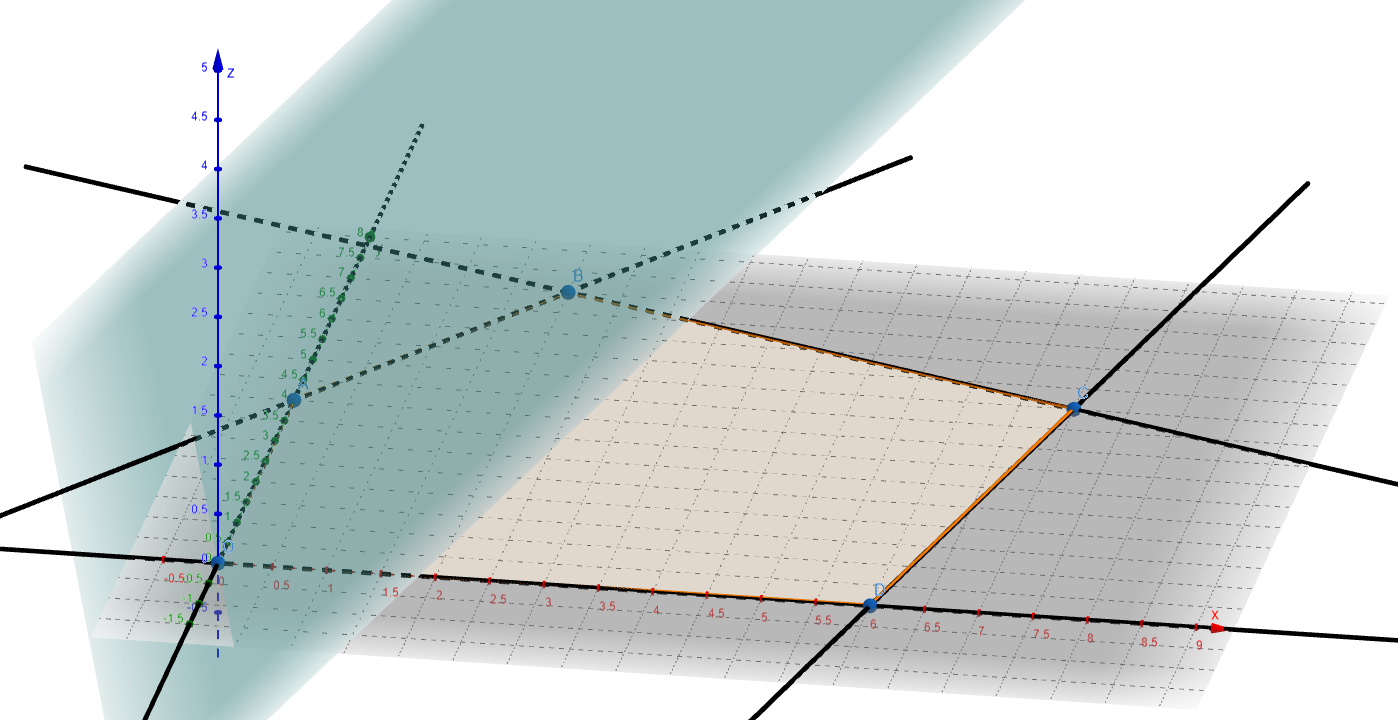
\includegraphics[width=0.45\linewidth]{example2.png}
    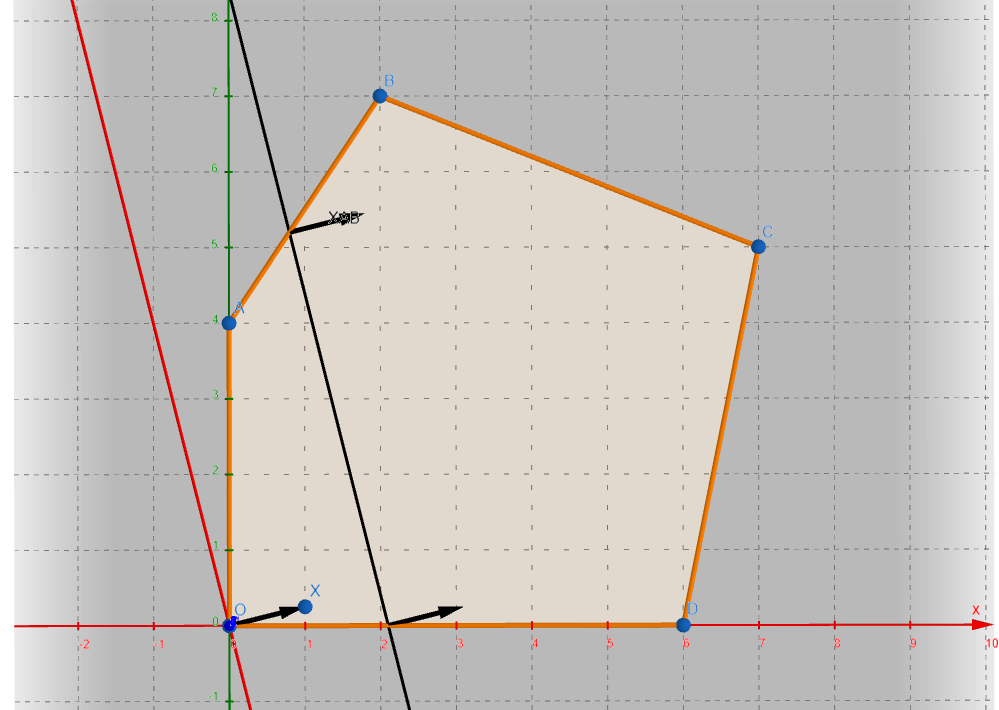
\includegraphics[width=0.45\linewidth]{Example3.png}
\end{figure}

ซึ่งถ้าใช้แนวคิดการไต่เขาตามให้ขนานกับแนวการไต่ระดับ จะพบว่าจุดสุดท้ายที่จะไต่ขึ้นไปได้คือจุด $C$ ด้วยการลากเส้นไต่ระดับขึ้นไปเรื่อย ๆ ดังรูป
\begin{figure}[h]
    \centering
    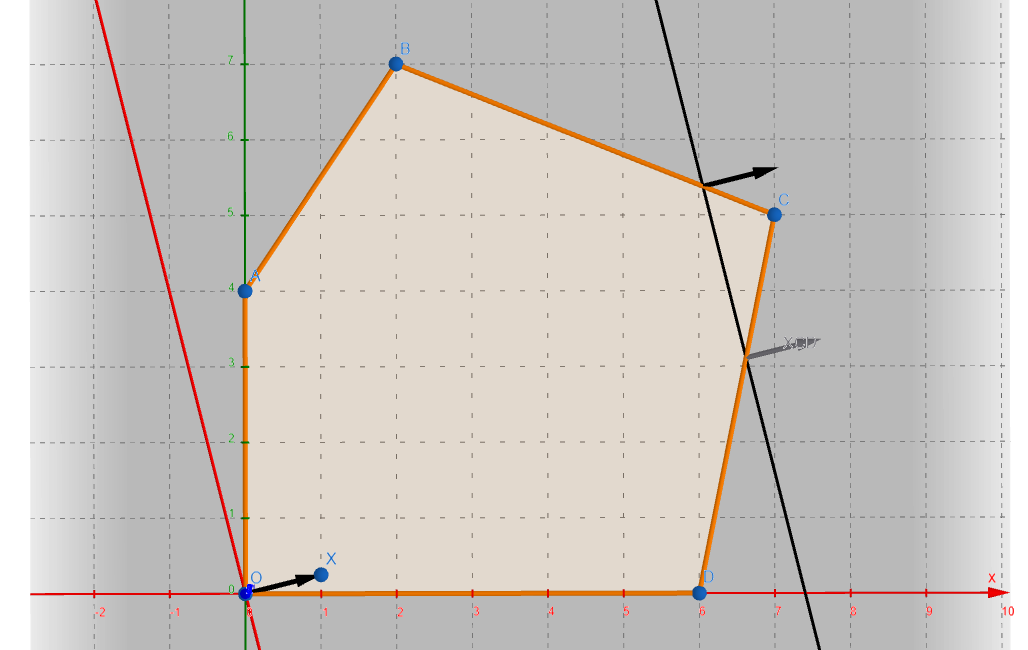
\includegraphics[width=0.75\linewidth]{Example4.png}
\end{figure}
และนอกจากวิธีการเลื่อนเส้นไต่ระดับแล้ว อีกวิธีที่ง่ายคือการลองแทนค่าทุกจุดยอดเพื่อคำนวณค่าจุดประสงค์แล้วเปรียบเทียบว่าค่าใดมากที่สุดหรือน้อยที่สุด

\begin{example}{โจทย์สำรวจคุณสมบัติ \ref{pro:linprogproperty}}{}
    พิจารณาโจทย์กำหนดการเชิงเส้น
    \begin{align*}
    \max  &\quad z=x+0.25y \\
    \text{subject to} &\quad x\geq0, \quad y\geq0\\
                &\quad y\leq1.5x+4\\
                &\quad y\leq-0.4x+7.8\\
                &\quad y\geq5x-30
    \end{align*}
    \begin{enumerate}
        \item จงแสดงว่าสมการเส้นตรงที่ระบุแนวหน้ากระดานการไต่ระดับ (เส้นที่เลื่อนตามรูปด้านบน) ที่ตัดแกน $y$ ที่ $y = c$ \underline{มีสมการเป็น $y=-4x + c$} กล่าวคือ แนวเส้นตรงที่มีความชัน $-4$ จะเป็นแนวที่ระนามมีค่าคงที่
        \item เมื่อพิจารณาบนแนวเส้นที่ทำให้ระนาบมีค่าคงที่ $y=-4x + 8$ เป็นตัวอย่าง จงหาจุดตัดของเส้นดังกล่าวกับเส้นตรง $y = 1.5x + 4$ กับเส้นตรง $y=0$
        \item จากจุดตัดที่ได้ในข้อที่ผ่านมา (ซึ่งมี 2 จุด) จงแสดงว่าทั้งสองจุดดังกล่าวให้ค่า $z=x + 0.25y$ \underline{เป็น $z = 2$}
        \item เมื่อพิจารณาบนแนวเส้นที่ทำให้ระนาบมีค่าคงที่ $y=-4x + c$ จงแสดงว่า \underline{ค่าคงที่ของระนาบคือ $z = 0.25c$}
    \end{enumerate}
\end{example}

\newpage
\begin{example}{แก้ปัญหากำหนดการเชิงเส้น 2 ตัวแปรด้วยการวาดภาพ}{}
    จงแก้โจทย์กำหนดการเชิงเส้นในตัวอย่าง \ref{ex:sampleLinProg} ด้วยวิธีวาดภาพ โดยพิจารณาค่าสูงสุดทั้งวิธีการไต่ระดับ และวิธีการลองแทนค่าทุกจุดยอด
\end{example}
\newpage
\begin{example}{แก้ปัญหากำหนดการเชิงเส้น 2 ตัวแปรด้วยการวาดภาพ}{}
    จงแก้โจทย์กำหนดการเชิงเส้นในตัวอย่าง \ref{ex:2varformulate} ด้วยวิธีวาดภาพ โดยพิจารณาค่าสูงสุดทั้งวิธีการไต่ระดับ และวิธีการลองแทนค่าทุกจุดยอด
\end{example}
\begin{solution}
    จากข้อที่ผ่านมา เราได้มาแล้วว่ากำหนดการเชิงเส้นคือ
    \begin{align*}
        \max  &\quad z=4000a + 1800b \\
        \text{s.t.} &\quad100a + 70b \leq 6000\\
                    &\quad800a + 600b \leq 100000\\
                    &\quad16a + 16b \leq 1000\\
                    &\quad a, b\geq0
        \end{align*}
    \begin{enumerate}[label=\textbf{ขั้นที่ \arabic*:}, align=left, labelwidth=5em, labelsep=1em, leftmargin=*, itemsep=16pt, topsep=0pt, parsep=0pt, partopsep=0pt]
    
    \item วาดรูปภาพเงื่อนไข โดยเรามี 3 เงื่อนไขดังนี้
        \begin{itemize}
            \item $100a + 70b = 6000$
            \item $800a + 600b = 100000$
            \item $16a + 16b = 1000$
        \end{itemize}
        ซึ่งทำได้โดยการหาจุดตัดแกน ซึ่งจะได้ดังนี้\\
        
        \begin{tabular}{|c|c|c|}
        \hline
            สมการ & จุดตัดแกน $x$ ($a$) & จุดตัดแกน $y$ ($b$) \\
            \hline
            $100a + 70b = 6000$ & 60 & 600/7 $\approx$ 85.71\\
            \hline
            $800a + 600b = 100000$ & 125 & $\approx$ 166.67\\
            \hline
            $16a + 16b = 1000$ & 62.5 & 62.5\\
            \hline
        \end{tabular}
        \begin{figure}[h]
            \centering
            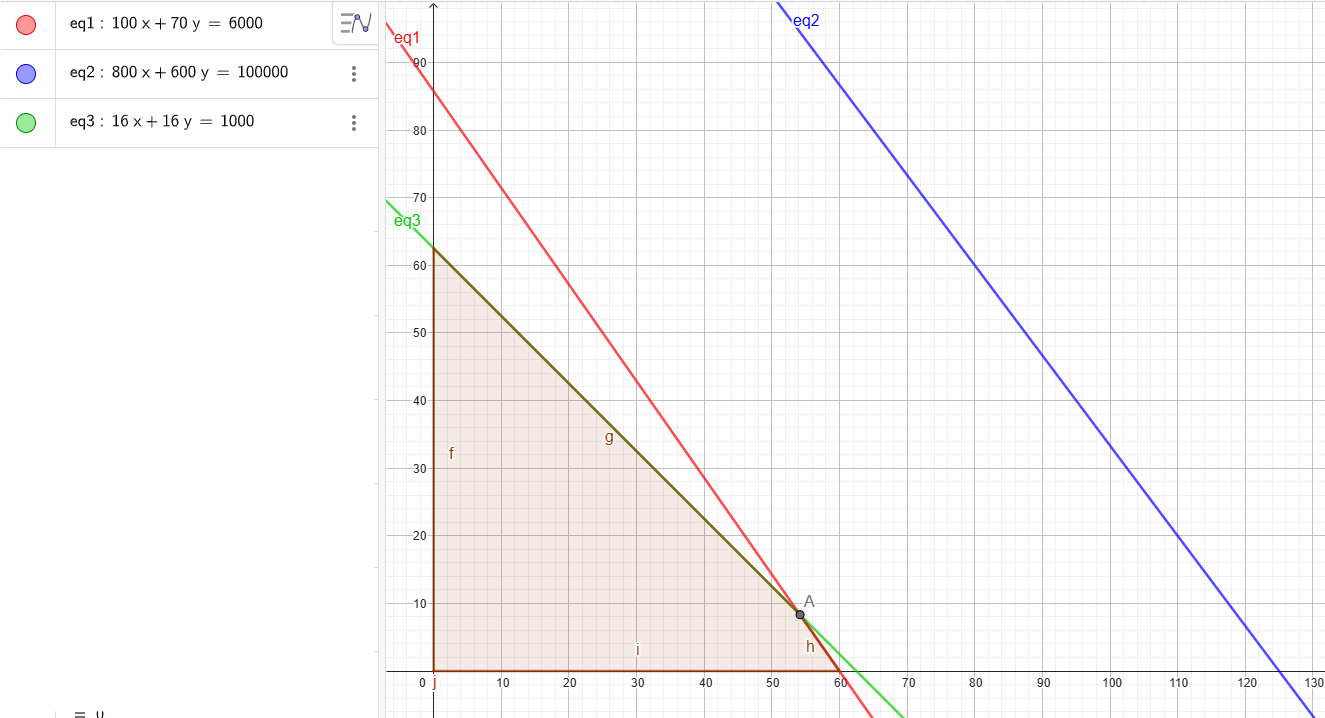
\includegraphics[width=0.75\linewidth]{ex113-1.png}
        \end{figure}
        และถ้าหาจุดตัดจากสมการที่ 1 และสมการที่ 3 ที่ตัดกันจะได้จุด $\approx(54.17,8.33)$

    \item แทนค่าจุดมุมลงในฟังก์ชันจุดประสงค์เพื่อหาค่าแล้วเปรียบเทียบกันว่าจุดใดให้ค่าจุดประสงค์มากที่สุด\\

    \begin{tabular}{c|c}
        $(a,b)$ & $\text{ยอดขาย} = 4000a + 1800b$ \\
        \hline
        $(0,62.5)\approx(0,62)$ & 111600 \\
        \hline
        $(54.17,8.33)\approx(54,8)$ & 230400 \\
        \hline
        $(60,0)$ & 240000 \\
        \hline
        $(0,0)$ & 0 \\
        \hline
    \end{tabular}

    \item สรุปคำตอบ จะได้ค่ายอดขายมากสุดเท่ากับ 240000 เกิดขึ้นที่จุด $(60,0)$ กล่าวคือผลิตกระบวนการที่ 1 เป็นจำนวน 60 เครื่อง และไม่ผลิตกระบวนการที่ 2 เลย
    \end{enumerate}
    \begin{remark}
        {โจทย์เพิ่ม}{}
        จะเห็นว่ากระบวนการที่ 2 ไม่ถูกใช้งานเลย ซึ่งอาจไม่เป็นที่พึงพอใจกับฝ่ายจัดซื้อที่ลงทุนไปกับการซื้อเครื่องมือสำหรับกระบวนการที่ 2 ไปแล้ว (เช่นกรณีกระบวนการที่ 2 เป็นเรื่องของเครื่องจักร) แต่เมื่อฝ่ายการตลาดทำการสำรวจเพิ่มเติม พบว่าเรายังสามารถทำสินค้า Y ให้มีภาพลักษณ์ที่พรีเมียมมากขึ้นเพื่อเปลี่ยนกลุ่มลูกค้าไปกลุ่มที่กำลังจ่ายสูงขึ้นได้ (เนื่องจากผลิตได้น้อยเมื่อเทียบกับ X ที่ผลิตได้ 4 ชิ้นต่อครั้งของกระบวนการที่ 1) ดังนั้นฝ่ายการตลาดจึงมาถามเราที่เป็นที่ปรึกษาทางธุรกิจว่าควรตั้งราคาขายสินค้า Y ให้อยู่ในช่วงราคาเท่าไหร่เพื่อให้ผลเฉลยที่ให้ยอดขายสูงสุดมาจากการใช้ทั้งเครื่องจักรของกระบวนการที่ 1 และเครื่องจักรของกระบวนการที่ 2\\

        นอกจากการปรับราคาแล้ว ยังมีทางเลือกอื่นใดบ้างในการปรับปรุงแบบจำลองให้ยังคงใช้ทั้ง 2 กระบวนการ โดยที่ไม่ต้องปรับราคา (แต่อาจจะได้ยอดขายรวมน้อยลงบ้างก็ยังยอมรับได้)
    \end{remark}
\end{solution}

\section{แนวคิดเบื้องต้นของวิธีซิมเพล็กซ์ (Simplex)}
ในหัวข้อที่แล้ว เราศึกษาวิธีการแก้ปัญหากำหนดการเชิงเส้นด้วยวิธีการรูปภาพ ซึ่งข้อจำกัดของวิธีการดังกล่าวคือเราจะสามารถแก้ปัญหาได้แค่กรณี 2 ตัวแปร และจริง ๆ แล้ว เราสามารถทำกับปัญหา 3 ตัวแปรก็ได้เช่นกันแต่จะวาดภาพยากกว่า เพราะต้องดูขอบเขตผลเฉลยใน 3 มิติ แต่ว่าถ้า 4 ตัวแปรเป็นต้นไปเราจะไม่สามารถวาดภาพได้อีกแล้ว ทำให้วิธีการดังกล่าวใช้ไม่ได้อีกต่อไป

\begin{figure}[h]
    \centering
    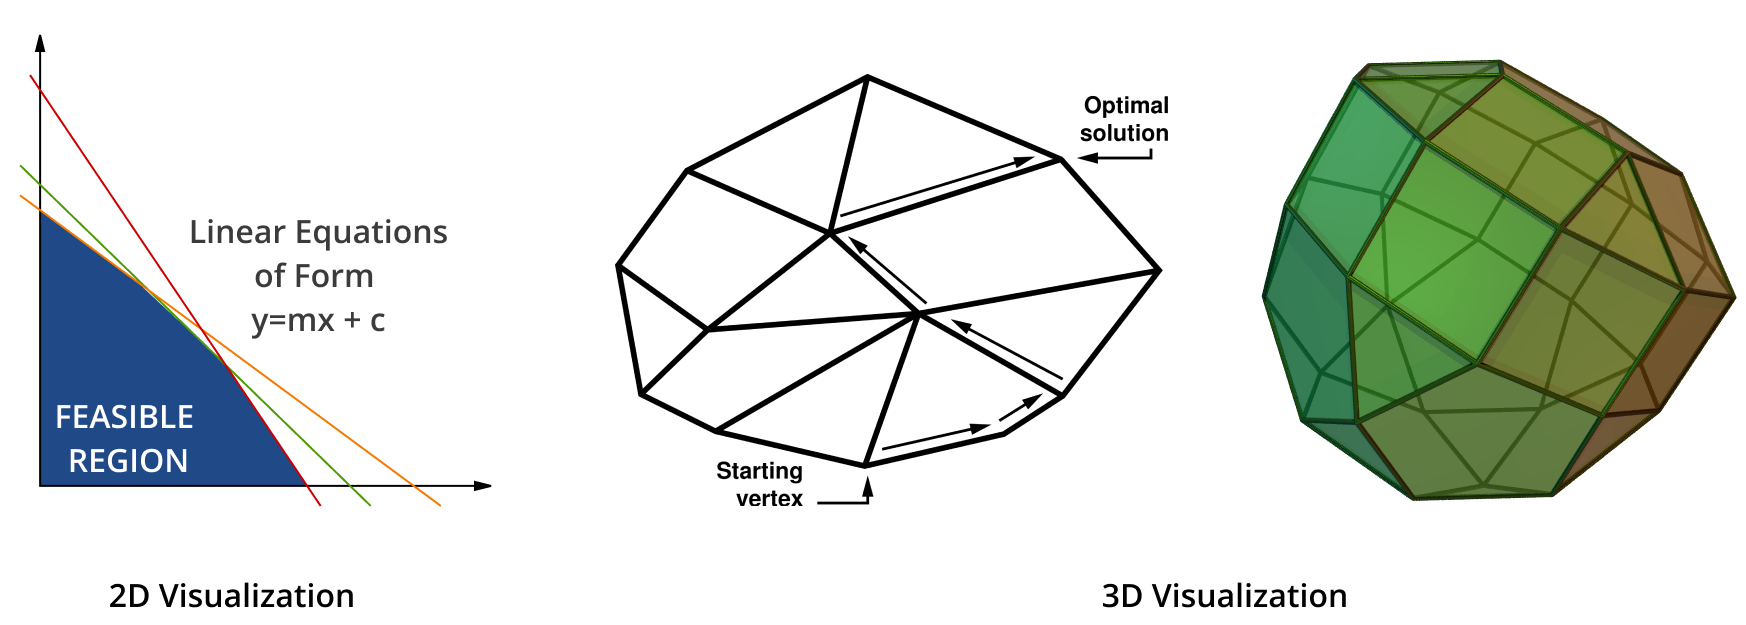
\includegraphics[width=1\linewidth]{simplex1.png}
\end{figure}

เครื่องมือที่จะใช้ในการแก้ปัญหากำหนดการเชิงเส้นสำหรับกรณีใด ๆ ก็ตามที่จะศึกษาในหัวข้อนี้คือวิธีซิมเพล็กซ์ (simplex method) ซึ่งเป็นกระบวนการในการใช้การดำเนินการทางเมทริกซ์เพื่อการเปลี่ยน pivot ที่จะให้ค่าสูงขึ้นเรื่อย ๆ ไล่ไปตามขอบของรูป โดยอาศัยคุณสมบัติตามที่เราได้ศึกษามาในกรณี 2 มิติว่าการเดินตามขอบบนบริเวณที่เป็นรูปนูน (convex) จะพาเราไปจุดผลเฉลยค่าสุดขีดได้แน่ ๆ

\begin{figure}[h]
    \centering
    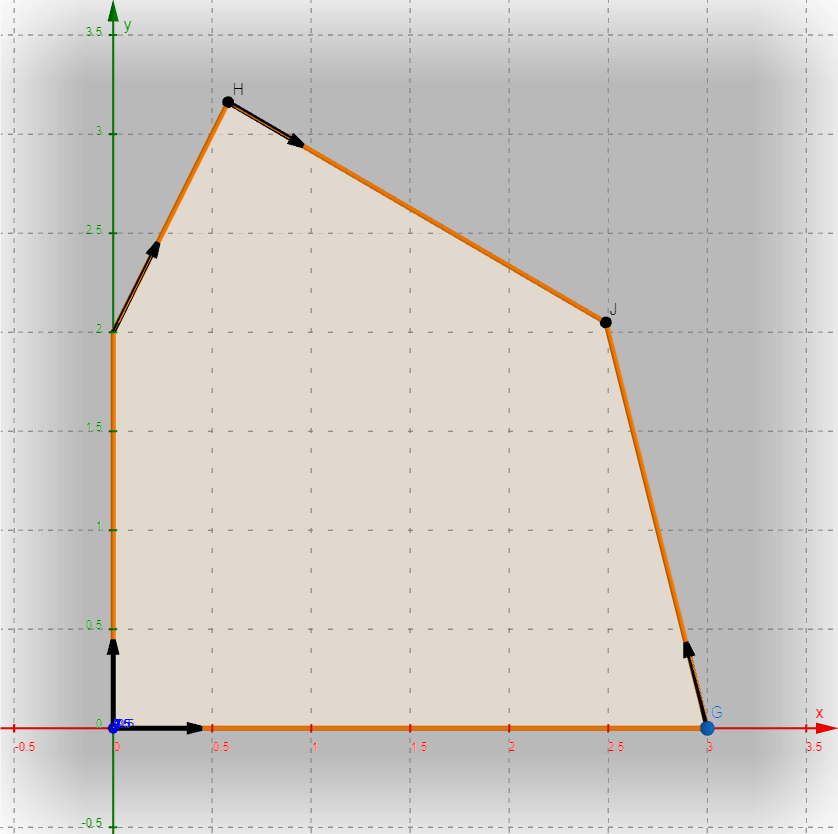
\includegraphics[width=0.5\linewidth]{simplex2.png}
\end{figure}

ทั้งนี้ สิ่งหนึ่งที่ต้องเน้นย้ำสำหรับขั้นตอนกระบวนการนี้คือสมมติฐานการเป็นรูปนูน เพราะอัลกอริทึมที่กำลังจะได้ศึกษาอาศัยการเดินตามเส้นขอบตามทิศทางที่มีค่าเพิ่มได้ ซึ่งเงื่อนไขที่การันตีการไปจุดผลเฉลยสุดขีดได้คือการเป็นรูปนูนที่ทำให้เราไต่ระนาบขึ้นได้เรื่อย ๆ เสมอตามรูปด้านบนที่เราสามารถเดินทางจากจุด $O$ ไปที่จุด $J$ ที่เป็นผลเฉลยได้ แต่ถ้ารูปพื้นที่เป็นไปได้ไม่ใช่รูปนูน อาจทำให้เกิดปัญหาที่เรียกว่าการติดค่าสุดขีดสัมพัทธ์ (local extrema) ตามรูปด้านล่าง ซึ่งถ้าเริ่มที่จุด $O$ จะเดินไปได้ไกลสุดแค่จุด $H$ หรือจุด $G$ เท่านั้นตามแนวคิดเบื้องต้นของ simplex แต่ในวิชานี้ เราจะโฟกัสไปแค่ที่โจทย์ที่พื้นที่ผลเฉลยเป็นรูปนูนอยู่แล้ว ดังนั้นนักศึกษาจึงไม่ต้องกังเรื่องสมมติฐานดังกล่าว

\begin{figure}[h]
    \centering
    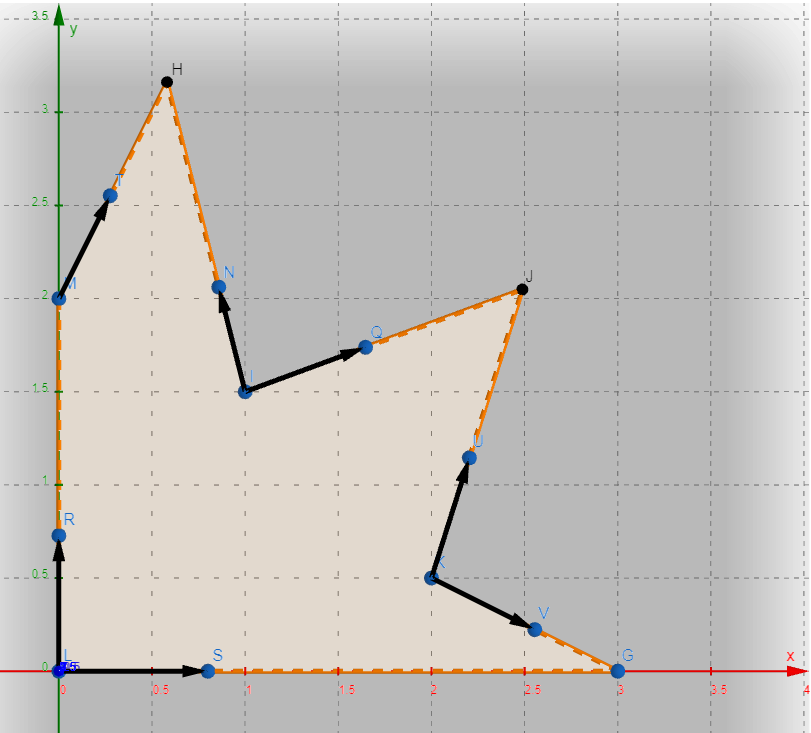
\includegraphics[width=0.4\linewidth]{simplex3.png}
\end{figure}

\subsubsection*{แนวคิดเชิงการคำนวณ (อ่านนอกเวลาเพิ่มเติม): wait revise again}
จะขอเริ่มจากตัวอย่างที่ง่ายเพื่อพาไปดูหลักการคิดทีละขั้น (สำหรับนักศึกษาที่สนใจ simplex method เลยสามารถข้ามหัวข้อนี้ได้) โดยปัญหากำหนดการเชิงเส้นที่จะพิจารณาคือ
\begin{align*}
    \max  &\quad 4x + y \\
    \text{subject to} &\quad x\geq0, \quad y\geq0\\
                &\quad x\leq 4\\
                &\quad y\leq 4
\end{align*}
และมีบริเวณการพิจารณาตามรูปด้านล่างนี้ ในรูปจะมีเวกเตอร์แนวการไต่ระดับของระนาบอยู่ และจะเห็นว่าจุด $(4,4)$ ควรเป็นจุดที่ให้ค่าสูงสุดแน่นอน
\begin{figure}[h]
    \centering
    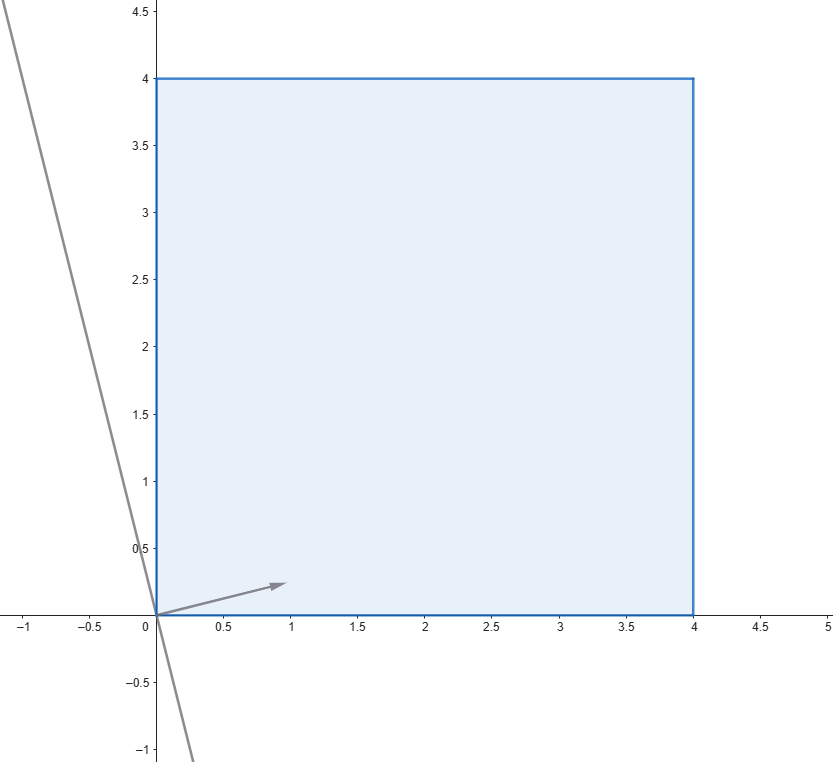
\includegraphics[width=0.4\linewidth]{basicSimplex1.png}
\end{figure}

แต่รูปแบบอสมการนั้นเป็นรูปแบบที่ไม่เหมาะกับการแก้ปัญหาในเชิงการคำนวณ ทำให้เราต้องเปลี่ยนรูปแบบการเขียนให้อยู่ในรูปแบบสมการเท่ากับ ซึ่งอาศัยคุณสมบัติของระบบจำนวนว่า
\begin{property}
    {เปลี่ยนอสมการเป็นสมการ}{}
    $$
    x \leq a \text{ ก็ต่อเมื่อ มีจำนวนจริง } s \text{ ที่เป็นบวกหรือศูนย์ที่ทำให้ } x+s = a
    $$
    ซึ่งตัวแปร $s$ ในที่นี้มีชื่อเรียกว่าตัวแปรส่วนเกิน (slack variable)
\end{property}

ซึ่งแน่นอนว่าตัวแปรส่วนเกินนี้จะเป็นเพียงแค่ตัวแปรที่เพิ่มเข้ามาในเงื่อนไข ไม่มีผลต่อค่าของฟังก์ชันจุดประสงค์ ดังนั้น เหล่าบรรดาเงื่อนไขอสมการจะต้องมีการเติมตัวแปรส่วนเกินเพื่อทำให้เป็นเงื่อนไขสมการได้ดังนี้
\begin{align*}
    \max  &\quad 4x + y + 0s_1 + 0s_2 \\
    \text{subject to} &\quad x, y, s_1, s_2\geq0\\
                &\quad x + s_1 = 4\\
                &\quad y + s_2 = 4
\end{align*}
หมายเหตุสำคัญตัวแปรทุกตัวจะต้องไม่ต่ำกว่า 0 เป็นเงื่อนไขบังคับ

ทีนี้ จะขอกล่าวถึงความหมายของตัวแปรส่วนเกินเชิงรูปภาพกันก่อนว่าคืออะไรในรูปภาพ ทั้งนี้อย่าลืมว่า simplex method คือการเดินตามขอบจากจุดยอดหนึ่งไปยังอีกจุดยอดหนึ่ง เพราะฉะนั้น เราจะพิจารณาแค่จุดตามขอบเท่านั้น รูปภาพด้านล่างนี้เป็นตัวอย่างค่าตัวแปรของจุดตามตำแหน่งขอบต่าง ๆ ซึ่งจะเห็นว่าตัวแปร $s_1$ ทีเป็นตัวแปรส่วนเกินของตัวแปร $x$ คือตัวแปรที่จะเติมเต็มให้ $x$ เดินไปถึงจุดยอดได้ และถ้าพิจารณาตามจุดยอดต่าง ๆ ก็จะพบว่าระหว่างตัวแปรของปัญหาและตัวแปรส่วนเกินที่คู่กันนั้นจะต้องมีอย่างน้อย 1 ตัวที่แปรที่มีค่าเป็น 0 ตัวอย่างเช่นการเดินตามขอบด้านล่างของรูปภาพในตัวอย่างนี้คือการแลกค่ากันระหว่าง $x$ และ $s_1$ โดยสมการ $x + s_1 = 4$ ที่จุดยอดซ้ายคือจุดที่ $x=0, s_1=4$ ในขณะที่จุดด้านขวาคือจุดที่ $x=4,s_1=0$ กล่าวคือ การเดินตามขอบของบริเวณที่เป็นไปได้จากจุดยอดไปอีกจุดยอดก็คือการพยายามแลกเปลี่ยนค่าของตัวแปรส่วนเกินให้เป็น 0 นั่นเอง

\begin{figure}[h!]
    \centering
    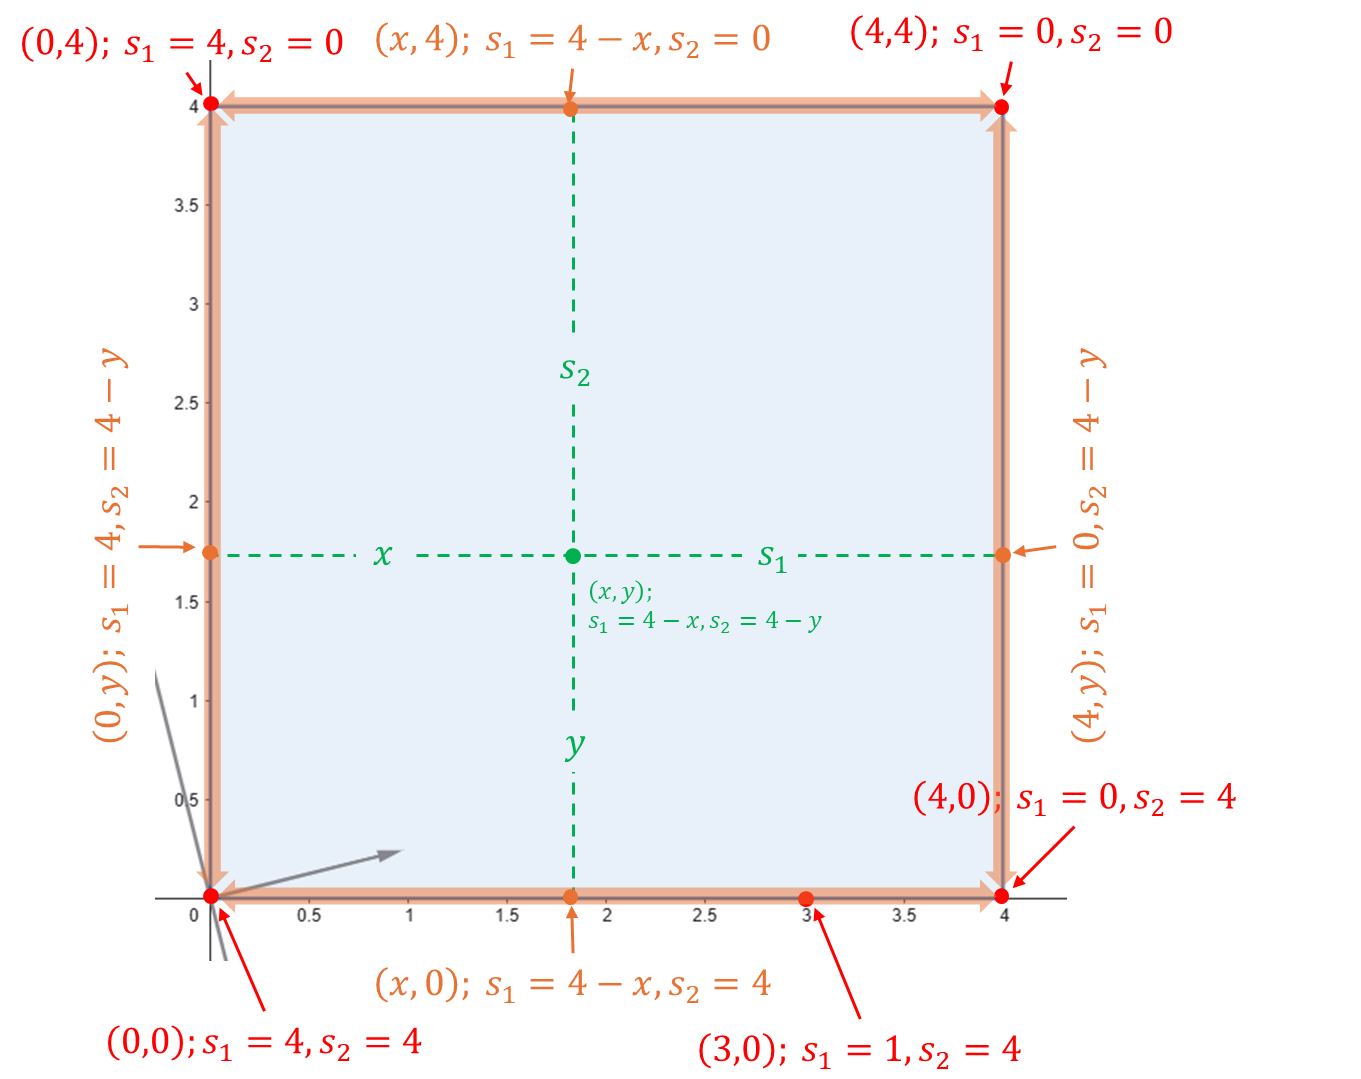
\includegraphics[width=0.7\linewidth]{basicSimplex2.png}
    \caption{Enter Caption}
    \label{fig:enter-label}
\end{figure}

จากที่กล่าวไปสักครู่ คือวิธีการเดินทางกรณีที่รู้แล้วว่าจะเดินตามขอบใด
คำถามต่อมาคือ เมื่อเรายืนอยู่ที่จุดยอดหนึ่ง จะรู้ได้อย่างไรว่าต้องเดินไปทางไหน ตัวอย่างเช่นถ้าเรากำลังยืนอยู่ที่จุด $(0,0)$ จะรู้ได้อย่างไรว่าต้องเดินตามขอบแนวตั้งไปที่ $(0,4)$ หรือตามขอบแนวนอนไปที่ $(4,0)$
ซึ่งถ้าอาศัยความรู้ในวิชาแคลคูลัสในแง่ขอการดูอัตราการเปลี่ยนแปลง จะทราบได้ทันทีว่าต้องเดินตามแนวแกน $x$ เพราะแนวการเดินใกล้กับเวกเตอร์ระบุทิศทางของระนาบมากที่สุด ซึ่งจริง ๆ แล้วก็สามารถดูได้โดยง่ายจากสัมประสิทธิ์ของตัวแปรในสมการ $z=4x+y+0s_1+0s_2$ ที่หมายความว่าการเดินตาม $x$ จะเปลี่ยนค่า $z$ เป็นระยะ 4 หน่วยเมื่อเพิ่ม $x$ ไป 1 หน่วย ในขณะที่ถ้าเดินตาม $y$ จะเปลี่ยนค่าแค่ 1 หน่วยเท่านั้น

ดังนั้น เราจึงสามารถตัดสินใจได้ว่าเราจะเดินตาม $x$ โดยจากเดิมที่ตรึง $x=0, y=0$ เราจะเปลี่ยนไปตรึง $s_1=0, y=0$ ซึ่งลักษณะการพิจารณาชุดตัวแปรในลักษณะนี้เราจะเรียกว่าชุดตัวแปรพื้นฐาน (basic variables) ซึ่งคือชุดตัวแปรที่จะถูกมองให้มีค่าเป็น 0 เพื่อใช้คำนวณค่าตัวแปรที่ไม่ใช่ตัวแปรพื้นฐาน (non-basic variables) กล่าวคือ จากเดิมที่เรากำหนดระบบเป็น $s_1 = 4 - x$ และ $s_2 = 4 - y$ โดยที่ $x=0, y=0$ จะโดนเปลี่ยนการพิจารณาระบบเป็น $x = 4 - s_1$ และ $s_2 = 4 - y$ โดยที่ $s_1=0, y=0$ ซึ่งเรียกการดำเนินการนี้ว่าการหมุนตัวแปรหลัก (pivot change) จากเดิมที่ $s_1, s_2$ เป็นตัวแปรหลัก (pivot variable) เราจะเปลี่ยนระบบให้ $x, s_2$ เป็นตัวแปรหลักแทน

สำหรับการดำเนินการหมุนตัวแปรหลัก ตัวแปรหลักจะไม่สามารถมีเพิ่มได้ ในตัวอย่างจะมีได้แค่ 2 ตัวแปร ดังนั้น การจะนำตัวแปรใหม่เข้ามาเป็นตัวแปรหลัก จึงต้องมีการนำ pivot ตัวเก่าออกหนึ่งตัว ซึ่งจะตามมาด้วยคำถามว่ารู้ได้อย่างไรว่าต้องเอา $s_1$ ออกจากการเป็นตัวแปรหลักแล้วนำ $x$ มาแทนที่
ซึ่งแนวคิดที่ใช้ในการเดินทางจริง ๆ เป็นเรื่องการเดินตามแนวตัวแปรหลักใหม่อย่างไรให้ไม่หลุดออกจากขอบ ซึ่งเห็นได้ชัดว่าถ้าเดินให้สั้นที่สุดเท่าที่จำเป็นเพื่อจะไปเจอขอบหนึ่งจะการันตีได้ว่าเราจะไม่เดินหลุดขอบแน่นอน ซึ่งคุณสมบัติของการเป็นรูปนูนคือจะไม่มีเส้นขอบใดที่ลากต่อแล้วตัดภายในพื้นที่เสมอดังรูปด้านล่างนี้
เพราะฉะนั้น ในทางปฏิบัติที่เราอาจไม่เห็นรูปภาพ เราจึงต้องเลือกการเดินที่สั้นที่สุดเอาไว้ก่อนเพื่อให้ไม่หลุดขอบถึงแม้จะไม่ใช่ทางที่เร็วที่สุดก็ตาม
และเมื่อทราบแล้วว่าต้องเดินไปชนขอบใด จึงค่อยพิจารณาว่าขอบนั้นเป็นขอบประชิดของตัวแปรส่วนเกินตัวไหน

\begin{figure}
    \centering
    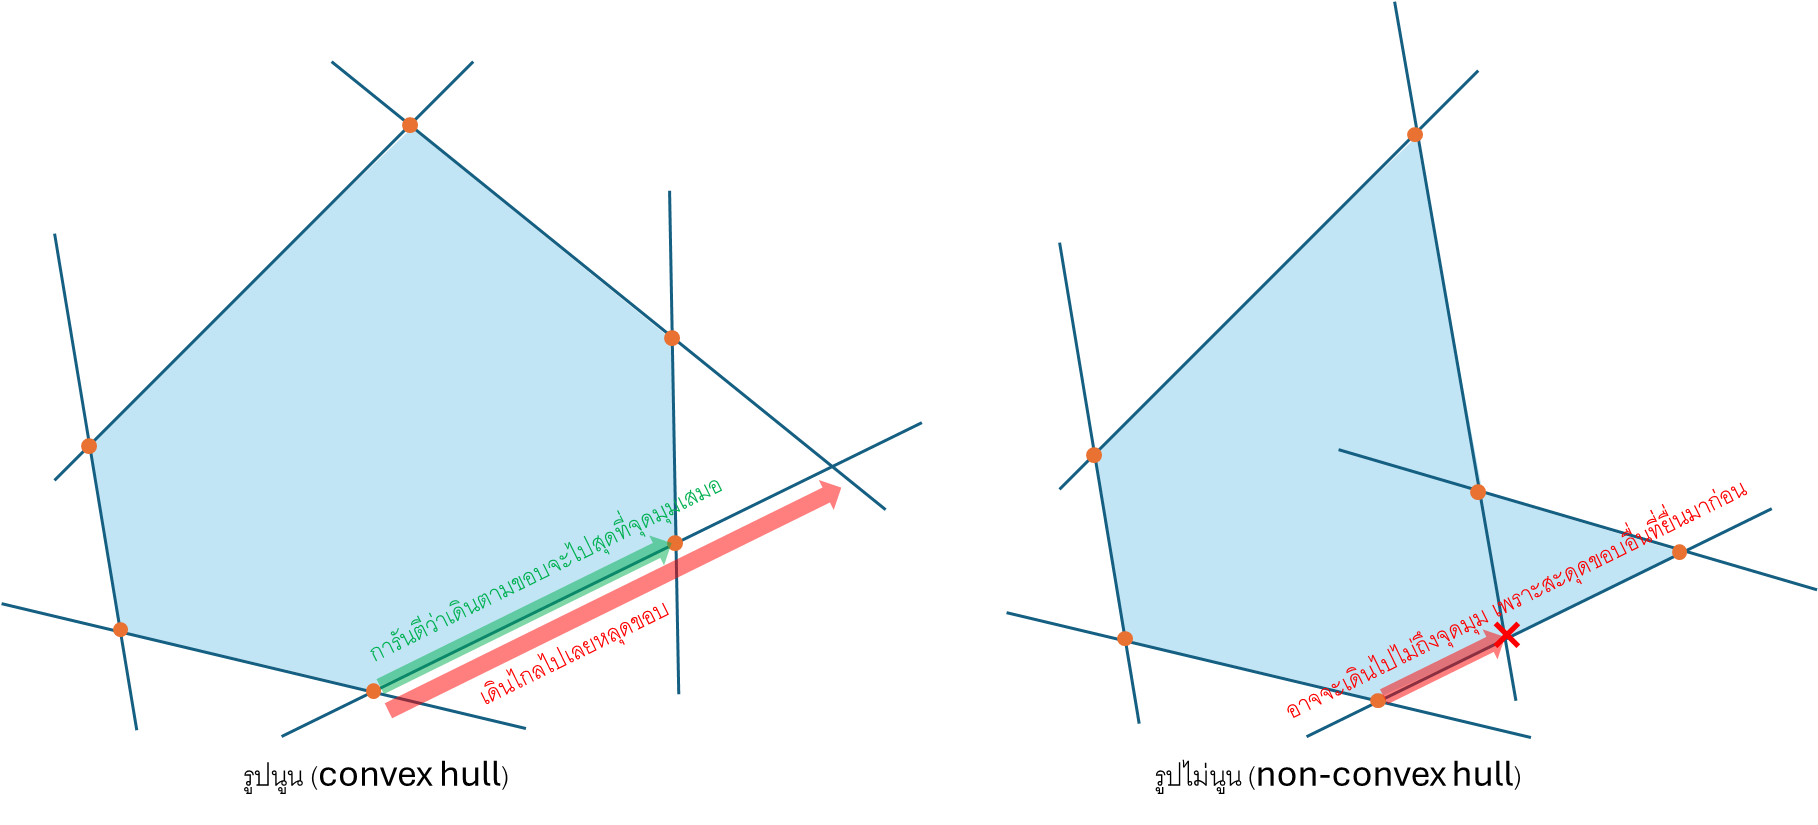
\includegraphics[width=0.8\linewidth]{SimplexConvexHull.png}
    \caption{Enter Caption}
    \label{fig:enter-label}
\end{figure}

จากตัวอย่างที่เรากำลังพิจารณาอยู่นั้น เราทราบแล้วว่าเราต้องเดินจาก $(0,0)$ ตามแนวตัวแปร $x$ แต่เนื่องจากรูปนี้ยังเป็นรูปอย่างง่ายจึงเห็นชัดว่ามีเส้นทางเดียวเท่านั้นที่ไปได้เมื่อบังคับให้เปลี่ยน $x$ คือเดินตามขอบแนวด้านล่าง และจะไปประชิดที่ขอบ $x=4$ ซึ่งคือขอบที่ตัวแปรส่วนเกิน $s_1=0$ จึงทำให้ทราบว่าเราต้องนำ $x$ ไปเป็นตัวแปรหลักแทน $s_1$ และให้ $s_1$ ทำหน้าที่ตัวแปรพื้นฐาน กล่าวคือ ตั้งให้ $s_1=0$ และ $y=0$ เป็นตัวแปรพื้นฐานและได้ว่า $x=4, y=0$ เพราะฉะนั้น จาก $z=4\times 0 + 1\times0 + 0\times 4 + 0\times 4 = 0$ ที่จุด $(0,0)$ จะได้ว่าค่าจุดประสงค์ ณ ปัจจุบันเปลี่ยนไปเป็น $z=4\times 4 + 1\times0 + 0\times 0 + 0\times 4 = 16$ และเราจะไม่เดินตาม $x$ อีกแล้ว

กล่าวคือตอนนี้ระบบเหลือแค่ปัญหา
\begin{align*}
    \max  &\quad y + 0s_2 + 16 \\
    \text{subject to} &\quad y, s_2\geq0\\
                &\quad y + s_2 = 4
\end{align*}
ซึ่งจะเห็นว่าเปรียบเสมือนการเดินตามแนว $y$ โดยที่จะเอา $y$ ไปเป็นตัวแปรหลักแทน $s_2$ จึงไปจบที่ขอบที่ $s_2=0$ ทำให้ได้ $y=4$ และจบด้วยการไม่สามารถปรับค่าตัวแปรไหนเพิ่มเติมได้อีกแล้ว จึงได้ว่า $(x,y) = (4,4)$ เป็นผลเฉลยที่ทำให้ได้ฟังก์ชันค่าจุดประสงค์มากที่สุด และเท่ากับ $z = 4\times 4 + 1\times 4 = 20$

ทั้งนี้ ขอสรุปขั้นตอนสำคัญของการทำ simplex method ดังนี้
\begin{enumerate}
    \item หา pivot ตัวใหม่: พิจารณาหาทิศทางที่ทำให้เปลี่ยนค่าได้เร็วสุดก่อน
    \item หา pivot ตัวที่จะถูกแทนที่: เมื่อทราบแนวการเปลี่ยนแล้ว ให้ดูว่าจุดที่ยืนอยู่ปัจจุบันมีเส้นทางไหนที่เดินแล้วถึงขอบเร็วสุดเพื่อป้องกันการหลุดนอกขอบ แล้วตัวแปรส่วนเกินของขอบนั้นจะโดนแทนที่กลายไปเป็นตัวแปรพื้นฐาน (ตัวแปรที่ถูกตั้งค่าให้เป็น 0)
    \item กำจัดตัวแปร pivot ใหม่ออกจากระบบ
    \item ทำวนไปเรื่อย ๆ จนไม่สามารถเปลี่ยนตัวแปรใด ๆ เพื่อเพิ่มค่าจุดประสงค์ได้อีกแล้ว
\end{enumerate}

\subsection{Simplex Method Algorithm}
ในการทำ simplex นั้นจะนิยมเขียนการคำนวณอยู่ในรูปแบบเมทริกซ์ที่เรียกว่า simplex tableau ดังนี้
\begin{center}
\renewcommand{\arraystretch}{1.4}
\begin{tabular}{|c|cccccc|c|}
\hline
\textbf{Pivot} & $x_1$ & $x_2$ & $\cdots$ & $x_n$ & $s_1$ & $\cdots$ & \textbf{RHS} \\
\hline
$x_{B_1}$ & $c_{11}$ & $c_{12}$ & $\cdots$ & $c_{1n}$ & $c_{1s_1}$ & $\cdots$ & $b_1$ \\
$x_{B_2}$ & $c_{21}$ & $c_{22}$ & $\cdots$ & $c_{2n}$ & $c_{2s_1}$ & $\cdots$ & $b_2$ \\
$\vdots$ & $\vdots$ & $\vdots$ & & $\vdots$ & $\vdots$ & & $\vdots$ \\
$x_{B_m}$ & $c_{m1}$ & $c_{m2}$ & $\cdots$ & $c_{mn}$ & $c_{ms_1}$ & $\cdots$ & $b_m$ \\
\hline
$Z$ & $z_1$ & $z_2$ & $\cdots$ & $z_n$ & $z_{s_1}$ & $\cdots$ & $z$ \\
\hline
\end{tabular}
\end{center}
โดยจะกล่าวละเอียดทีละขั้น โดยมีขั้นตอนดังนี้

\begin{algorithm}
    {Simplex Method}{}
    ก่อนอื่น ตัวแปรทุกตัวต้องไม่ติดลบ ($x_i \geq 0$) และเงื่อนไขอยู่ในรูปแบบซึ่งก้อนตัวแปรอยู่ฝั่งซ้ายและค่าคงที่อยู่ฝั่งขวาโดยที่ค่าคงที่ต้องไม่ติดลบ
    \begin{enumerate}[label=\textbf{ขั้นที่ \arabic*.}, align=left, labelwidth=5em, labelsep=1em, leftmargin=*, itemsep=0pt, topsep=0pt, parsep=0pt, partopsep=0pt]
 
  \item \textbf{แปลงปัญหาให้อยู่ในรูปแบบมาตรฐาน (Standard Form)}  
  \begin{itemize}[itemsep=0pt, topsep=0pt, parsep=0pt, partopsep=0pt]
    \item เป้าหมายต้องอยู่ในรูปแบบ \textbf{Maximize $Z = c_1x_1 + c_2x_2 + \dots + c_nx_n$}
    \item ข้อจำกัดต้องอยู่ในรูป \textbf{สมการ} โดยการเพิ่มตัวแปรประเภท \textit{slack, surplus, artificial} ตามความเหมาะสม
  \end{itemize}

  \item \textbf{เขียน Simplex Tableau แรก}  
  \begin{itemize}[itemsep=0pt, topsep=0pt, parsep=0pt, partopsep=0pt]
    \item สร้างตารางแสดงสัมประสิทธิ์ของตัวแปรในแต่ละ constraint
    \item เพิ่มแถวของสมการ $Z$ และค่าคงที่ (RHS)
  \end{itemize}

  \item \textbf{เลือกตัวแปรที่จะเข้าสู่ฐาน (Entering Variable)}  
  \begin{itemize}[itemsep=0pt, topsep=0pt, parsep=0pt, partopsep=0pt]
    \item เลือกตัวแปรที่มีสัมประสิทธิ์ในแถว $Z$ น้อยที่สุด (ติดลบมากที่สุด)
    \item ถ้าไม่มีค่าสัมประสิทธิ์ใดติดลบในแถว $Z$: หยุดได้เลยเพราะได้คำตอบที่เหมาะสมแล้ว
  \end{itemize}

  \item \textbf{ทำ Minimum Ratio Test เพื่อเลือกตัวแปรที่จะออกจากฐาน (Leaving Variable)}  
  \begin{itemize}[itemsep=0pt, topsep=0pt, parsep=0pt, partopsep=0pt]
    \item สำหรับแต่ละแถวที่ตัวแปรเข้ามามีสัมประสิทธิ์เป็นบวก ให้คำนวณ:
    \[
    \text{Ratio} = \frac{\text{RHS}}{\text{ค่าสัมประสิทธิ์ของตัวแปรเข้าใหม่}}
    \]
    \item เลือกแถวที่ให้ค่า Ratio ต่ำสุด
    \item ถ้าไม่มี Ratio ใดสามารถคำนวณได้ (ทุกสัมประสิทธิ์ ≤ 0) → ปัญหา \textbf{ไม่จำกัดคำตอบ} (Unbounded)
  \end{itemize}

  \item \textbf{ทำ Pivot เพื่ออัปเดต Tableau}  
  \begin{itemize}[itemsep=0pt, topsep=0pt, parsep=0pt, partopsep=0pt]
    \item ทำให้ตำแหน่ง Pivot (จุดตัดระหว่างแถวเข้าและออก) มีค่าเป็น 1
    \item ปรับแถวอื่นให้ค่าของตัวแปรเข้ามาในคอลัมน์นั้นเป็น 0
  \end{itemize}

  \item \textbf{ทำซ้ำขั้นตอนที่ 3–5 จนกว่าจะไม่มีสัมประสิทธิ์ติดลบในแถว $Z$}

  \item \textbf{อ่านคำตอบจาก Tableau สุดท้าย}  
  \begin{itemize}[itemsep=0pt, topsep=0pt, parsep=0pt, partopsep=0pt]
    \item ตัวแปรในฐานจะมีค่าตรงกับ RHS
    \item ตัวแปรที่ไม่อยู่ในฐานจะมีค่าเป็น 0
    \item ค่า $Z$ ที่เหมาะสมที่สุดอยู่ในมุมขวาล่างของแถว $Z$
  \end{itemize}

\end{enumerate}
\end{algorithm}

\subsubsection{กรณีที่ 1: เงื่อนไขมีแต่ $\leq$ (จุดกำเนิดเป็น basic feasible solution)}
กรณีนี้เป็นกรณีที่ง่ายที่สุด เพราะเป็นกรณีที่เริ่มกระบวน simplex ได้ทันทีที่จุดกำเนิดโดยไม่ต้องมีการปรับแต่งอะไรก่อนหน้า
ในการอธิบายวิธีการของกรณีนี้ จะขอใช้ตัวอย่างดังนี้
\begin{align*}
    \max \quad & 3x + 5y \\
    \text{subject to} \quad
    & x \geq 0, \quad y \geq 0 \\
    & x \leq 4 \\
    & y \leq 6 \\
    & 3x + 2y \leq 18
\end{align*}

\subsubsection*{ขั้นที่ 1: แปลงปัญหาให้อยู่ในรูปแบบมาตรฐาน (Standard Form)}
\begin{itemize}
  \item เป้าหมาย $\max 3x + 5y$ อยู่ในรูป \textbf{การเพิ่มค่า (Maximization)} อยู่แล้ว
  \item แต่ถ้าเป้าหมายเป็น \textbf{Minimization}, ต้องแปลงเป็น \textbf{Maximization} โดยเปลี่ยนเครื่องหมาย:
  \[
  \text{Minimize } Z = c_1x_1 + c_2x_2 \quad \Rightarrow \quad \text{Maximize } -Z = -c_1x_1 - c_2x_2
  \]
    \item ทุกตัวแปรต้องมีเงื่อนไข \textbf{ไม่ติดลบ}:
  \[
  x_i, s_i, a_i \geq 0
  \]
    ถ้าติดลบ ให้เปลี่ยนเป็นตัวแปรใหม่ $x_{new} = -x$ (แต่ในกรณีนี้ยังไม่มี)
  \item ข้อจำกัดทั้งหมดต้องเขียนในรูปสมการ (equalities) โดยข้อจำกัดแบบ $\leq$, ให้เพิ่ม \textbf{ตัวแปรส่วนเกิน (Slack Variable)} $s_i$: $a_1x_1 + a_2x_2 \leq b \quad \Rightarrow \quad a_1x_1 + a_2x_2 + s_i = b$

\end{itemize}
\begin{example}{เปลี่ยนรูปมาตรฐานกรณี 1}{}
    จงเปลี่ยนปัญหา
    \begin{align*}
        \max \quad & 3x + 5y \\
        \text{subject to} \quad
        & x \geq 0, \quad y \geq 0 \\
        & x \leq 4 \\
        & y \leq 6 \\
        & 3x + 2y \leq 18
    \end{align*}
    ให้อยู่ในรูปมาตรฐาน
\end{example}

\begin{center}
    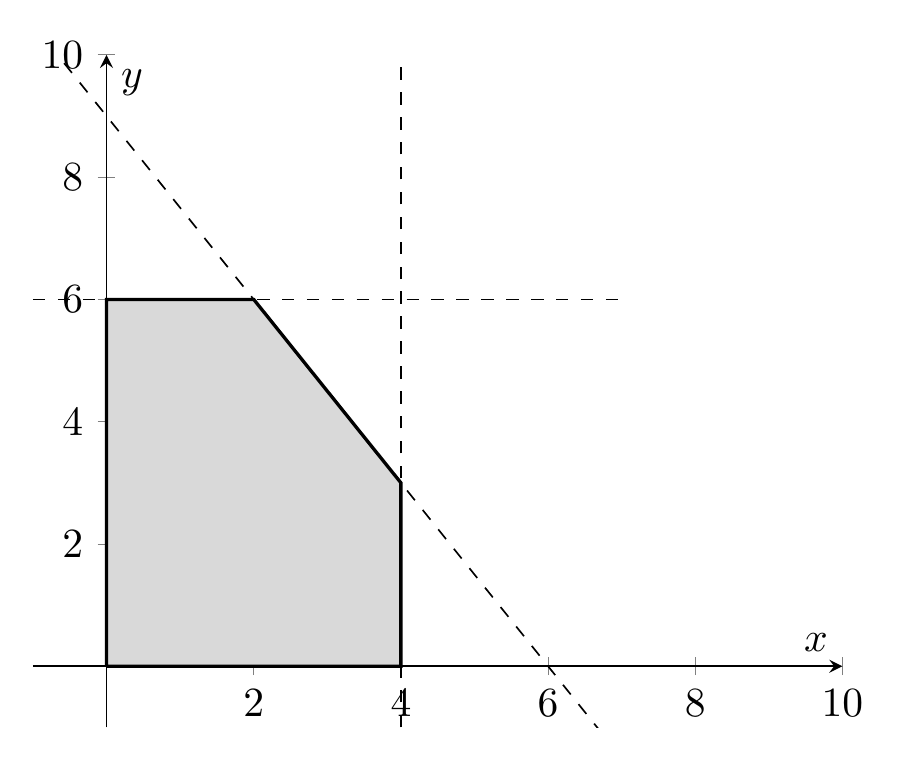
\begin{tikzpicture}[scale=1.5]
\begin{axis}[
  axis lines=middle,
  xmin=-1, xmax=10,
  ymin=-1, ymax=10,
  % xtick=0...20,
  % ytick=0...20,
  xlabel={$x$}, ylabel={$y$},
]
\addplot[black, dashed, domain=-1:7] {6};
\addplot[black, dashed, domain=-1:7] {-1.5*x + 9};
\addplot[black, dashed] coordinates {(4, -1) (4, 10)}; % vertical line x=4
\addplot[black, thick, fill=gray!30] coordinates {(0,0) (0,6) (2,6) (4,3) (4,0) (0,0)};
\end{axis}
\end{tikzpicture}
\end{center}


\subsubsection*{ขั้นที่ 2: เขียน Simplex Tableau แรก}
โดยให้กลุ่มตัวแปรส่วนขาดเป็นตัวแปร pivot ของระบบก่อน และให้ตัวแปรตัดสินใจเป็นตัวแปรพื้นฐาน กล่าวคือเราให้จุดกำเนิดเป็นผลเฉลยตั้งต้น
และนอกจากนั้น เราจะให้แถวสุดท้ายมีค่าเป็นค่าติดลบของสัมประสิทธิ์แต่ละตัวแปรในฟังก์ชันจุดประสงค์ $z$ และ RHS มีค่าเป็น 0
\begin{example}
    {Initial Simplex Tableau}{}
    จากรูปมาตรฐานที่ได้จากตัวอย่างที่ผ่านมา จะเขียน Simplex tableau เริ่มต้นได้ดังนี้
    \begin{center}
    \renewcommand{\arraystretch}{1.4}
        \begin{tabular}{|c|ccccc|c|}
            \hline
            \textbf{Pivot} & $x$ & $y$ &  $s_1$ & $s_2$ & $s_3$ & \textbf{RHS} \\
            \hline
            $ $ & $ $ & $ $  & $ $ & $ $ & $ $ & $ $ \\
            $ $ & $ $ & $ $  & $ $ & $ $ & $ $ & $ $ \\
            $ $ & $ $ & $ $  & $ $ & $ $ & $ $ & $ $ \\
            $ $ & $ $ & $ $  & $ $ & $ $ & $ $ & $ $ \\
            \hline
            $z$ & $ $ & $ $  & $ $ & $ $ & $ $ & $ $ \\
            \hline
        \end{tabular}
    \end{center}
\end{example}

\newpage
หมายเหตุ: จริง ๆ แล้วเรายังมีอีกคอลัมน์นึงที่ถูกซ่อนไว้คือคอลัมน์ของตัวแปรจุดประสงค์ $z$ ซึ่งจะสามารถเขียนได้เป็น
    \begin{center}
    \renewcommand{\arraystretch}{1.4}
        \begin{tabular}{|c|cccccc|c|}
            \hline
            \textbf{Pivot} & $z$ & $x$ & $y$ &  $s_1$ & $s_2$ & $s_3$ & \textbf{RHS} \\
            \hline
            $ $ &$0$ & $ $ & $ $  & $ $ & $ $ & $ $ & $ $ \\
            $ $ &$0$ & $ $ & $ $  & $ $ & $ $ & $ $ & $ $ \\
            $ $ &$0$ & $ $ & $ $  & $ $ & $ $ & $ $ & $ $ \\
            \hline
            $z$& $1$ & $ $ & $ $  & $ $ & $ $ & $ $ & $ $ \\
            \hline
        \end{tabular}
    \end{center}
แต่เนื่องจากไม่ว่าจะดำเนินการในขั้นอื่น ๆ ต่อไปอย่างไร คอลัมน์นี้จะไม่มีทางเปลี่ยนแปลงแน่นอน ดังนั้นจึงละการเขียนคอลัมน์นี้ไว้
\begin{property}
    {คำถาม}{}
    \begin{enumerate}
    \item ทำไมแถวของฟังก์ชันจุดประสงค์ถึงต้องใช้ค่าติดลบของสัมประสิทธิ์ และทำไมฝั่ง RHS ถึงต้องมีค่าเป็น 0
    \item การเป็น Pivot ของตัวแปรหมายถึงอะไร
    \item อะไรในตารางที่บอกเราว่าปัจจุบันเรายืนอยู่ที่จุด $(0,0)$
\end{enumerate}
\end{property}
\newpage
\subsubsection*{ขั้นที่ 3: เลือกตัวแปรที่จะเข้าสู่ฐาน (Entering Variable)}
จากตำแหน่งที่ยืนอยู่ ณ ปัจจุบัน สิ่งที่เราต้องหาในขั้นตอนถัดไปคือควรจะเดินไปตามทางไหน ซึ่งแน่นอนว่าเราไม่ได้ระบุการเดินแบบบอกทิศการเดินชัดเจน (ถึงแม้ในกรณีนี้เราจะทราบว่าการเดินไปตามเวกเตอร์ $(3,5)$ จะเป็นทิศที่ไต่ขึ้นได้เร็วสุดก็ตาม)
เพราะหลักการของ simplex คือการเดินตามขอบ
เพราะฉะนั้นเราจึงบอกทิศการเดินแบบคร่าว ๆ ว่าจะเดินไปตามแนวแกนของตัวแปรใดก็เพียงพอแล้ว (ในที่นี้คือแนวแกน $x$ หรือแนวแกน $y$)

วิธีการที่จะเลือกว่าเราควรเดินไปทิศทางใด คือการดูสัมประสิทธิ์ของตัวแปรนั้นที่อยู่ในฟังก์ชันจุดประสงค์
\begin{example}
    {การเลือกตัวแปรฐานใหม่}{}
    จากฟังก์ชันจุดประสงค์ (ในปัจจุบัน) $z = 3x + 5y + 0s_1 + 0s_2 + 0s_3$ ถ้า แต่ละตัวแปรมีค่าเปลี่ยนไป +1 แล้วค่า $z$ จะมีค่าเปลี่ยนไปเท่าไหร่บ้าง และการเปลี่ยนตัวแปรใดทำให้เพิ่มค่า $z$ ได้มากที่สุด
\end{example}

\newpage

\subsubsection*{ขั้นที่ 4: เลือกตัวแปรที่จะออกจากฐาน (Leaving Variable)}

\begin{center}
    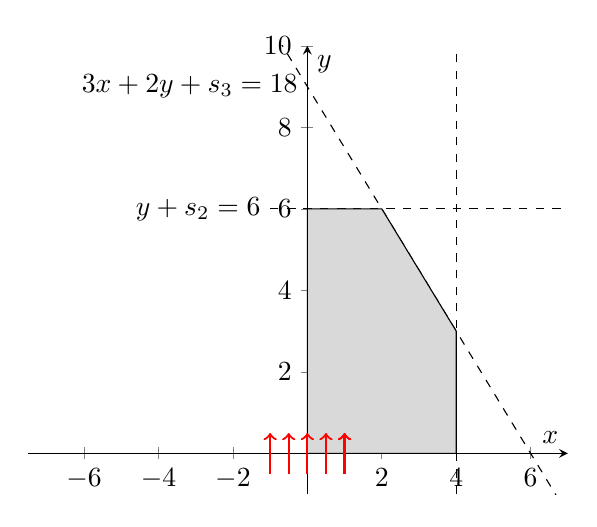
\begin{tikzpicture}
\begin{axis}[
  axis lines=middle,
  xmin=-7.5, xmax=7,
  ymin=-1, ymax=10,
  % xtick=0...20,
  % ytick=0...20,
  xlabel={$x$}, ylabel={$y$},
]
\addplot[black, dashed, domain=-1:7] {6};
\addplot[black, dashed, domain=-1:7] {-1.5*x + 9};
\addplot[black, dashed] coordinates {(4, -1) (4, 10)}; % vertical line x=4
\addplot[black, fill=gray!30] coordinates {(0,0) (0,6) (2,6) (4,3) (4,0) (0,0)};
\addplot[red, thick, ->] coordinates {(-1,-0.5) (-1,0.5)};
\addplot[red, thick, ->] coordinates {(-0.5,-0.5) (-0.5,0.5)};
\addplot[red, thick, ->] coordinates {(-0,-0.5) (-0,0.5)};
\addplot[red, thick, ->] coordinates {(0.5,-0.5) (0.5,0.5)};
\addplot[red, thick, ->] coordinates {(1,-0.5) (1,0.5)};
\addplot[red, thick, ->] coordinates {(1,-0.5) (1,0.5)};
\addplot[] coordinates {(-1, 6)}
node[pos=0.7, anchor=east] {$y+s_2 = 6$};
\addplot[] coordinates {(0, 9)}
node[pos=0.7, anchor=east] {$3x+2y+s_3 = 18$};
\end{axis}
\end{tikzpicture}
\end{center}

ณ ขั้นตอนนี้ เราทราบแล้วว่าเรากำลังจะเอาตัวแปร $y$ เข้ามาเป็นตัวแปรฐานใหม่ เพราะการเดินตามแนวแกน $y$ ให้การเปลี่ยนค่า $z$ ได้มากที่สุด
ซึ่งจากรูปภาพเราจะเห็นว่าจะมีเพียงขอบด้านซ้าย (เดินไปตามแกน $y$) เท่านั้นที่เป็นเส้นทางการเดินเดียวจากจุด $(0,0)$

คำถามต่อมาคือเดินควรไกลแค่ไหนถึงจะมั่นใจได้ว่าเดินไปถึงจุดมุมของบริเวณแน่ ๆ
ซึ่งถ้าเดินสั้นไปจะเดินไม่ถึงจุดมุม แต่ถ้าเดินไกลไปก็จะเลยจุดมุม
เพราะฉะนั้น เราจึงใช้ตัวแปรส่วนขาดเป็นตัวบอกว่าขอบของตัวแปรส่วนขาดใดอยู่ใกล้ที่สุด (ในกรณีอื่นอาจมีได้หลายเส้นทาง แต่เราก็จะเลือกอันที่ใกล้ที่สุดอยู่)
หรือกล่าวคือ เรากำลังจำลองว่าจะต้องเปลี่ยนค่า $y$ เท่าไหร่เพื่อให้ตัวแปรส่วนขาดของเส้นดังกล่าวมีค่าเป็น 0
\begin{example}
    {การเลือกตัวแปรเพื่อออกจากฐาน}{}
    จากรูปจะเห็นว่าถ้าเราเดิน จะไปพบได้ 2 เส้นเท่านั้นคือเส้นของ $s_2$ และเส้นของ $s_3$ จงหาค่า $y$ ของแต่ละเส้นที่ทำให้ตัวแปรส่วนขาดของเส้นดังกล่าวมีค่าเป็น 0 (สุดท้ายจะได้ว่าต้องเดินไปเส้นของ $s_2$)
    และเราจะสามารถเขียนแสดงผลลัพธ์ดังกล่าวในรูปแบบ simplex tableau ได้อย่างไร 
\end{example}
\newpage

\subsubsection*{ขั้นที่ 5: ทำ Pivot Row Operation เพื่ออัปเดต Tableau}

\begin{center}
    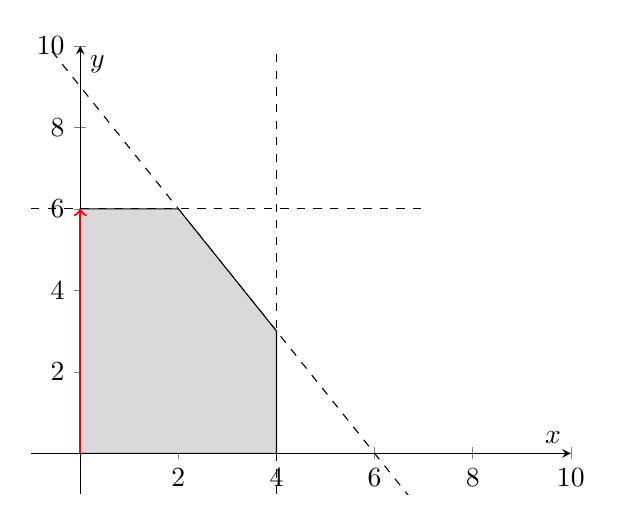
\begin{tikzpicture}
\begin{axis}[
  axis lines=middle,
  axis on top=false,
  xmin=-1, xmax=10,
  ymin=-1, ymax=10,
  % xtick=0...20,
  % ytick=0...20,
  xlabel={$x$}, ylabel={$y$},
]
\addplot[black, dashed, domain=-1:7] {6};
\addplot[black, dashed, domain=-1:7] {-1.5*x + 9};
\addplot[black, dashed] coordinates {(4, -1) (4, 10)}; % vertical line x=4
\addplot[black, fill=gray!30] coordinates {(0,0) (0,6) (2,6) (4,3) (4,0) (0,0)};
\addplot[red, thick, ->] coordinates {(0,0) (0,6)};
\end{axis}
\end{tikzpicture}
\end{center}

ตามความหมายในวิชาพีชคณิตเชิงเส้นเรื่องการแก้ระบบสมการเชิงเส้นนั้น pivot หมายถึงคอลัมน์ในเมทริกซ์สัมประสิทธิ์ที่มีสมาชิกเป็น 1 อยู่ตัวเดียว (เรียกว่า pivot element) และที่เหลือเป็น 0 ล้วน โดยในแต่ละแถวจะมี pivot element ได้ไม่เกิน 1 ตัว ซึ่งจากการที่เราบังคับให้ $s_2$ ออกจากการเป็นฐาน และนำ $y$ เข้ามาเป็นฐานแทน $s_2$ จึงต้องการให้ตาราง simplex อันใหม่มีหน้าตาดังนี้
    \begin{center}
    \renewcommand{\arraystretch}{1.4}
        \begin{tabular}{|c|ccccc|c|}
            \hline
            \textbf{Pivot} & $x$ & $y$ &  $s_1$ & $s_2$ & $s_3$ & \textbf{RHS} \\
            \hline
            $s_1$ & $*$ & $*$  & $1$ & $0$ & $0$ & $*$ \\
            $s_2$ & $*$ & $*$  & $0$ & $1$ & $0$ & $*$ \\
            $s_3$ & $*$ & $*$  & $0$ & $0$ & $1$ & $*$ \\
            \hline
            $z$   & $*$ & $*$  & $0$ & $0$ & $0$ & $*$ \\
            \hline
        \end{tabular}
        $\Longrightarrow$
        \begin{tabular}{|c|ccccc|c|}
            \hline
            \textbf{Pivot} & $x$ & $y$ &  $s_1$ & $s_2$ & $s_3$ & \textbf{RHS} \\
            \hline
            $s_1$ & $*$ & $0$  & $1$ & $*$ & $0$ & $*$ \\
            $y$   & $*$ & $1$  & $0$ & $*$ & $0$ & $*$ \\
            $s_3$ & $*$ & $0$  & $0$ & $*$ & $1$ & $*$ \\
            \hline
            $z$   & $*$ & $0$  & $0$ & $*$ & $0$ & $*$ \\
            \hline
        \end{tabular}
    \end{center}

\begin{example}
    {การเปลี่ยน pivot ของระบบ}{}
    แปลง simplex tableau ให้เป็นของระบบ pivot $s_1$, $y$ และ $s_3$ และให้เหตุผลว่าทำไมระบบปัจจุบันถึงแสดงสถานะว่ากำลังยืนอยู่ที่จุด $(0,6)$
\end{example}
\newpage
\subsubsection*{ขั้นที่ 6: วนซ้ำขั้นที่ 3-5 จนกว่าจะไม่มีสัมประสิทธิ์ติดลบในแถวของ $z$}
\begin{example}
    {ทำต่อ}{}
    ทำขั้นตอนที่ 3-5 วนจนกว่าจะจบกระบวนการ และแปลผลตารางสุดท้าย (ขั้นที่ 7)
\end{example}
\newpage
\begin{example}
    {}{}
    ใช้วิธี simplex หาผลเฉลยของกำหนดการเชิงเส้น
    \begin{align*}
        \max \quad & 4x + 2y \\
        \text{subject to} \quad
        & x \geq 0, \quad y \geq 0 \\
        & x \leq 2 \\
        & y \leq 3 \\
        & x - y \leq 1\\
        & x + y \leq 4
    \end{align*}
\end{example}
\newpage

\subsubsection{กรณีที่ 2: เงื่อนไขมี $\geq$ ที่อาจจะทำให้จุดกำเนิดไม่เป็น basic feasible solution}
ในบางกรณี เราอาจพบเงื่อนไขที่ทำให้จุดกำเนิดไม่ใช่ feasible solution เลยทำให้ไม่สามารถดำเนินการ simplex ได้ทันทีเหมือนกรณีที่ 1
ซึ่งกรณีดังกล่าวคือกรณีที่อสมการเงื่อนไขเขียนในรูป $ax + by \geq c$ โดยที่ $c \geq 0$ ซึ่งจะเห็นได้โดยง่ายว่าจุด $(0,0)$ ไม่เป็น feasible solution สำหรับเงื่อนไขนี้
แต่ถึงแม้เราจะใช้วิธีการการเพิ่มตัวแปรส่วนขาดเข้าไป ตัวอย่างเช่นสมการ $-3x + 5y \geq 4$ เมื่อเราทำการเพิ่มตัวแปรส่วนขาดเข้าไป จะได้สมการเป็น $-3x + 5y = 4 + s$ เมื่อ $s \geq 0$ หรือก็คือสมการ $-3x + 5y - s = 4$\footnote{หนังสือบางเล่มจะเรียกว่า\textbf{ตัวแปรส่วนเกิน} เพราะมองในลักษณะ $-3x + 5y - s = 4$ โดยที่ $s$ เป็นส่วนเกินของฝั่งที่มีค่ามากกว่า ทำให้เราต้องลบออกเพื่อให้ได้สมการ แต่ในมุมของผู้เขียนจะขอมองในลักษณะของตัวแปรส่วนขาดทั้งหมด แล้วใช้การย้ายข้างสมการแทน}
ซึ่งจะเห็นว่าถ้าให้ $x=0$ และ $y=0$ แล้วจะได้ว่า
$$
4 = -3x + 5y - s = -s \Longrightarrow s = -4 \ngeq 0
$$
กล่าวคือ เราไม่สามารถให้ $x$ และ $y$ เป็นตัวแปร non-basic ได้เหมือนกรณีที่ 1 

วิธีแก้ปัญหาคือเราจะเพิ่มตัวแปรเข้าระบบไปอีกตัว เพื่อปรับดุลสมการให้สามารถเริ่ม basic feasible solution ที่จุดกำเนิดได้ ซึ่งตัวแปรที่ถูกเพิ่มเข้ามานี้ถูกเรียกว่า \textbf{ตัวแปรจำลอง} (artificial variable) โดยจะได้สมการตัวอย่างเป็น
$$
-3x + 5y - s + A = 4 \text{ โดยที่ } A\geq 0
$$
และจะให้ตัวแปรจำลองเป็นตัวแปรพื้นฐาน และ $x,y,s$ มีค่าเป็น 0
โดยในขั้นตอนนี้ เราได้ basic feasible solution เริ่มต้นเป็นตัวแปรจำลอง ($A$) ซึ่งมีค่าเป็นบวก (ในที่นี้คือ $A=4$)  
แต่เป้าหมายของเราในการทำ Simplex method คือการกำจัดตัวแปรจำลองออกไปจากระบบในที่สุด เพราะตัวแปรจำลองนี้ไม่ได้มีความหมายในทางปฏิบัติ แต่เป็นเพียงตัวช่วยชั่วคราวในการเริ่มต้นหาคำตอบที่เหมาะสมที่สุดของระบบสมการ

การดำเนินการจากนี้เรียกกันโดยทั่วไปว่า \textbf{Simplex Method ระยะที่หนึ่ง (Phase I Simplex Method)} ซึ่งมีขั้นตอนการดำเนินงานดังต่อไปนี้:

\begin{enumerate}
    \item หลังจากเพิ่มตัวแปรจำลองในแต่ละสมการที่มีเงื่อนไข $\geq$ เรียบร้อยแล้ว เราจะกำหนดฟังก์ชันวัตถุประสงค์ชั่วคราว (Phase I Objective) ให้เป็นการหาผลรวมของตัวแปรจำลองทั้งหมดที่ถูกเพิ่มเข้าไป และเป้าหมายของขั้นตอนนี้คือการทำให้ผลรวมของตัวแปรจำลองมีค่าเท่ากับศูนย์ให้ได้ กล่าวคือเราสร้างฟังก์ชันวัตถุประสงค์ชั่วคราว (Phase I Objective) ดังนี้:
\[
\text{Minimize}\quad W = \sum (\text{ตัวแปรจำลองทั้งหมด})
\]

สำหรับตัวอย่างนี้จะได้เป็น
\[
\text{Minimize}\quad W = A
\]

    \item ใช้วิธี Simplex กับฟังก์ชันวัตถุประสงค์ชั่วคราวนี้ (Minimize $W$) และดำเนินการแปลงแถว (Pivot) ไปเรื่อย ๆ จนกว่าจะได้ตัวแปรจำลองจะออกจากฐานทั้งหมด

\begin{itemize}
    \item หากสามารถทำให้ฟังก์ชันวัตถุประสงค์ชั่วคราว $W=0$ ได้สำเร็จ แสดงว่าปัญหานี้มี feasible solution เดิมจริง และสามารถไปสู่ขั้นตอน Phase II ได้
    \item หากไม่สามารถทำให้ $W=0$ ได้ (เช่น $W>0$ เสมอ) แสดงว่าปัญหานี้ไม่มี feasible solution (infeasible problem) ไม่จำเป็นต้องดำเนินการต่อ
\end{itemize}

    \item เมื่อได้ $W=0$ แล้ว (กำจัดตัวแปรจำลองหมดแล้ว) เราจะดำเนินการต่อในขั้นที่สอง (\textbf{Phase II}) โดยกลับไปใช้ฟังก์ชันวัตถุประสงค์จริงของปัญหาเดิม และเริ่มทำ Simplex method ตามปกติจนได้คำตอบสุดท้าย
\end{enumerate}

\noindent
สรุปได้ว่าในกรณีที่ 2 นี้ การใช้ตัวแปรจำลอง (Artificial variable) และวิธีการ Simplex Phase I จะช่วยให้เราสามารถเริ่มต้นแก้ปัญหาการกำหนดการเชิงเส้นได้ แม้ว่าเงื่อนไขของปัญหาจะทำให้จุดกำเนิดไม่สามารถเป็น basic feasible solution ตั้งต้นได้ก็ตาม

\begin{example}
    {}{}
    ใช้วิธี simplex หาผลเฉลยของกำหนดการเชิงเส้น
    \begin{align*}
        \max \quad & 4x + 5y \\
        \text{subject to} \quad
        & x \geq 0, \quad y \geq 0 \\
        & -3x + 5y \geq 4\\
        & x + 2y \leq 8
    \end{align*}
\end{example}
\begin{solution}
    \begin{enumerate}[label=\textbf{ขั้นที่ \arabic*:}, align=left, labelwidth=5em, labelsep=1em, leftmargin=*, itemsep=16pt, topsep=0pt, parsep=0pt, partopsep=0pt]
    \item ปรับสมการให้อยู่ในรูปมาตรฐาน
        \begin{itemize}
            \item เนื่องจาก $(0,0)$ \textbf{ไม่}สอดคล้องเงื่อนไข $-3x + 5y \geq 4$ (แทนค่าแล้วได้ $0\geq 4$ ซึ่งเป็นเท็จ) เป็นจริง ดังนั้นจึงต้องเติมตัวแปรส่วนเกินและตัวแปรจำลอง ได้เป็น $-3x + 5y - s_1 + a_1 = 4$ โดยที่ $s_1, a_1 \geq 0$ โดยที่ให้ $a_1$ เป็นตัวแปรฐาน และ $x,y,s_1 = 0$ ในขั้นตั้งต้น
            \item เนื่องจาก $(0,0)$ สอดคล้องเงื่อนไข $3x + 2y \leq 8$ (แทนค่าแล้วได้ $0 \leq 8$ ซึ่งเป็นจริง) ดังนั้นจึงเติมตัวแปรส่วนขาดเข้าไปเท่านั้น ได้เป็น $x + 2y + s_2 = 8$ โดยที่ให้ $s_2$ เป็นตัวแปรฐานและ $x,y=0$
        \end{itemize}
        และเนื่องจากว่ามีตัวแปรจำลอง จึงต้องตั้งฟังก์ชันจุดประสงค์ชั่วคราวมให้เป็นการหาค่าต่ำสุดของผลรวมตัวแปรจำลอง กล่าวคือ $\min a_1$ แต่เนื่องจากเรากำลังจะทำ simplex จึงต้องปรับปัญหาให้เป็นการหาค่าสูงสุดด้วยการคูณ $-1$ เข้าไปได้เป็น $\max W = -a_1$ จึงได้ปัญหา Phase 1 ออกมาเป็น
        \begin{align*}
            \max \quad & W = -a_1 \\
            \text{subject to} \quad
            & x, y, s_1, s_2, a_1 \geq 0 \\
            & -3x + 5y -s_1 + a_1 = 4\\
            & x + 2y + s_2 = 8
        \end{align*}

    \newpage
    \item ตั้งตารางซิมเพล็กซ์ของตัวแปรจำลอง ได้เป็น
    \begin{center}
        \begin{tabular}{|c|ccccc|c|}
            \hline
            \textbf{Pivot} & $x$ & $y$ &  $s_1$ & $s_2$ & $a_1$ &  \textbf{RHS}  \\
            \hline
            $a_1$ & $-3$ & $5$  & $-1$ & $0$ & $1$ & $4$ \\
            $s_2$ & $1$ & $2$  & $0$ & $1$ & $0$ & $8$ \\
            \hline
            $W$   & $0$ & $0$  & $0$ & $0$ & $1$ & $0$ \\
            \hline
        \end{tabular}
    \end{center}
    และทำการกำจัดตัวแปรจำลองออกจากจุดประสงค์ (การเอาตัวแปรอื่นมาพิจารณา) เพื่อให้คอลัมน์ $a_1$ มีแถวของ $a_1$ เป็น 1 เพียงคนเดียว (เป็น pivot element ที่ตำแหน่งอื่นเป็น 0 ล้วน) ซึ่งทำได้โดยดำเนินการตามแถว $(-1)R_1 + R_3 \rightarrow R_3$ จะได้สมาชิกในแถวที่ $R_3$ ใหม่คำนวณได้ดังนี้
    \begin{itemize}
        \item คอลัมน์ $x$: $(-1)(-3) + 0 = 3$
        \item คอลัมน์ $y$: $(-1)(5) + 0 = -5$
        \item คอลัมน์ $s_1$: $(-1)(-1) + 0 = 1$
        \item คอลัมน์ $s_2$: $(-1)(0) + 0 = 0$
        \item คอลัมน์ $a_1$: $(-1)(1) + 1 = 0$
        \item คอลัมน์ $RHS$: $(-1)(4) + 0 = -4$
    \end{itemize}
    จึงได้ตารางซิมเพล็กซ์ตั้งต้นดังนี้ \textbf{(ถ้าในข้อสอบถามหาตารางตั้งต้น ต้องตอบตารางนี้ เพราะำคอลัมน์ $a_1$ ในตารางก่อนหน้ายังไม่อยู่ในรูปแบบ Pivot column)}
    \begin{center}
        \begin{tabular}{|c|ccccc|c|}
            \hline
            \textbf{Pivot} & $x$ & $y$ &  $s_1$ & $s_2$ & $a_1$ &  \textbf{RHS}  \\
            \hline
            $a_1$ & $-3$ & $5$  & $-1$ & $0$ & $1$ & $4$ \\
            $s_2$ & $1$ & $2$  & $0$ & $1$ & $0$ & $8$ \\
            \hline
            $W$   & $3$ & $-5$  & $1$ & $0$ & $0$ & $-4$ \\
            \hline
        \end{tabular}
    \end{center}
    \begin{remark}{การหาแถว $W$ อีกแบบ}{}
        เราสามารถหาแถว $W$ ได้แบบเร็วๆ โดยการนำสมการเงื่อนไขที่มีตัวแปรจำลองมาจัดรูปให้ตัวแปรจำลองอยู่ฝั่งหนึ่ง และตัวแปรที่เหลืออยู่อีกฝั่ง แล้วนำไปแทนค่าใน $W$ เช่นในเงื่อนไขที่ 1 ของตัวอย่างนี้คือ $-3x + 5y -s_1 + a_1 = 4$ และจัดรูปได้เป็น $a_1 = 3x - 5y + s_1 + 4$ แล้วนำไปแทนใน $W$ จะได้
        $$
        W = -a_1 = - (3x - 5y + s_1 + 4) = -3x + 5y - s_1 -4
        $$
        และย้ายข้างได้รูปแบบ $W +3x - 5y + s_1 = -4$ ทำให้เขียนสัมประสิทธิ์ได้เป็น $$3\quad-5\quad1\quad0\quad0\quad|\quad-4$$
    \end{remark}

    และทำกระบวนการ simplex ไปจนกว่าตัวแปรจำลองจะออกจากตัวแปรฐานทั้งหมด โดยจากตารางจะได้ว่าต้องให้ $y$ เป็นตัวแปรเข้าฐาน และเมื่อหาอัตราส่วนเพื่อเลือกตัวแปรขาออกจากฐานตามตารางด้านล่าง จะได้ว่าต้องใช้ $a_2$ ออกจากฐาน

    \begin{center}
        \begin{tabular}{|c|ccccc|c|c|}
            \hline
            \textbf{Pivot} & $x$ & $y$ &  $s_1$ & $s_2$ & $a_1$ &  \textbf{RHS} & อัตราส่วน  \\
            \hline
            $a_1$ & $-3$ & $5$  & $-1$ & $0$ & $1$ & $4$ & $4/5= 0.8$ \\
            $s_2$ & $1$ & $2$  & $0$ & $1$ & $0$ & $8$ & $8/2= 4$ \\
            \hline
            $W$   & $3$ & $-5$  & $1$ & $0$ & $0$ & $-4$ & \\
            \hline
        \end{tabular}
    \end{center}

    ดำเนินการตามแถวเพื่อเปลี่ยน pivot โดยใช้ $R_1/5$, $(-2/5)R_1 + R_2 \rightarrow R_2 $ และ $(1)R_1 + R_3 \rightarrow R_3 $ จะได้
    \begin{center}
        \begin{tabular}{|c|ccccc|c|}
            \hline
            \textbf{Pivot} & $x$ & $y$ &  $s_1$ & $s_2$ & $a_1$ &  \textbf{RHS}  \\
            \hline
            $y$ & $-3/5$ & $1$  & $-1/5$ & $0$ & $1/5$ & $4/5$ \\
            $s_2$ & $11/5$ & $0$  & $2/5$ & $1$ & $-2/5$ & $32/5$ \\
            \hline
            $W$   & $0$ & $0$  & $0$ & $0$ & $1$ & $0$ \\
            \hline
        \end{tabular}
    \end{center}
    ซึ่งตารางใหม่ไม่สามารถอัพเดตเพิ่มเติมได้อีกแล้ว และตัวแปรจำลองถูกกำจัดออกจากตัวแปรฐานได้ทั้งหมด และได้ $W=0$ จึงได้ว่าสามารถทำ simplex phase 2 ต่อได้โดยใช้ชุดสัมประสิทธิ์ที่ได้จาก phase 1
    \begin{center}
        \begin{tabular}{|c|cccc|c|}
            \hline
            \textbf{Pivot} & $x$ & $y$ &  $s_1$ & $s_2$ &  \textbf{RHS}  \\
            \hline
            $y$ & $-3/5$ & $1$  & $-1/5$ & $0$ & $4/5$ \\
            $s_2$ & $11/5$ & $0$  & $2/5$ & $1$ & $32/5$ \\
            \hline
            $z$   & $-4$ & $-5$  & $0$ & $0$ & $0$ \\
            \hline
        \end{tabular}
    \end{center}

    \begin{remark}{ความหมายของผลที่ได้จาก Phase 1}{}
        ผลที่ได้จากการทำ simplex phase 1 คือการพยายามหาจุดผลเฉลยตั้งต้น (basic feasible solution) ซึ่งจากเดิมเราสามารถเริ่มได้โดยง่ายที่จุด $x=0, y=0$ แต่ว่าในกรณีที่มีเงื่อนไขที่ทำให้จุดดังกล่าวไม่สอดคล้อง (เช่นเงื่อนไข $-3x + 5y \geq 4$) เราจึงจำเป็นต้องเพิ่มตัวแปรจำลองเพื่อจำลองการเดินทางจากจุด $(0,0)$ ไปที่จุดมุมตั้งต้นที่ใกล้ที่สุด ซึ่งจากตารางสุดท้ายที่ได้มาจาก phase 1 เราได้ระบบสมการ
        \begin{align*}
            -\frac{3}{5}x + y - \frac{1}{5}s_1 &= \frac{4}{5}\\
            \frac{11}{5}x + \frac{2}{5}s_1 + s_2 &= \frac{32}{5}
        \end{align*}
        โดยที่ $x = 0, s_1=0$ (เพราะไม่ใช่ฐาน) ซึ่งเมื่อแก้ระบบสมการหาค่าตัวแปรฐาน จะได้ $y=4/5$ และ $s_2 = 32/5$ ซึ่งหมายถึง เราหาจุดผลเฉลยตั้งต้นได้เป็นจุด $(x,y) = (0, 4/5)$ และใช้ระบบของจุดนี้เพื่อไปแก้หาค่าสูงสุดของ $Z$ ต่อได้
    \end{remark}
    
    \item ดำเนินการ simplex ได้ตามปกติ (ทิ้งไว้ให้เป็นแบบฝึกหัดเพิ่มเติมเพื่อทบทวนการดำเนินการ simplex)
    \end{enumerate}
\end{solution}

\subsubsection{กรณีที่ 3: เงื่อนไขมี $=$ ซึ่งทำให้ feasible ไม่เป็น region เต็มมิติ}
\begin{example}
    {}{}
    ใช้วิธี simplex หาผลเฉลยของกำหนดการเชิงเส้น
    \begin{align*}
        \max \quad & 2x + 15y \\
        \text{subject to} \quad
        & x \geq 0, \quad y \geq 0 \\
        & -3x + 5y \leq 15\\
        & 2x + 5y \leq 40\\
        & 4x -5y = 20
    \end{align*}
\end{example}
\newpage
\begin{example}
    {โจทย์ผสม}{}
    ใช้วิธี simplex หาผลเฉลยของกำหนดการเชิงเส้น
    \begin{align*}
        \min \quad & -1840x - 1720y \\
        \text{subject to} \quad
        & x \geq 0, \quad y \geq 0 \\
        & 2x+y \leq 1800\\
        & 2x + 2y \geq 1400\\
        & x -2y = 100
    \end{align*}
\end{example}
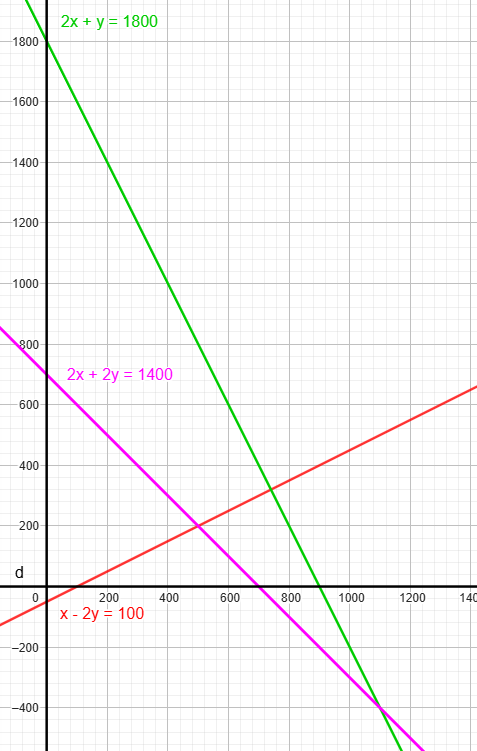
\includegraphics[width=0.5\linewidth]{ex-simplex-mix.png}


\newpage
\section{การแก้ปัญหาด้วย Excel Solver}

\subsection*{สถานการณ์จำลอง}
โรงงานผลิตน้ำผลไม้แห่งหนึ่งมีผลิตภัณฑ์ 4 ชนิด ได้แก่ น้ำส้ม (A), น้ำแอปเปิ้ล (B), น้ำองุ่น (C) และน้ำเสาวรส (D) โดยการผลิตแต่ละชนิดต้องใช้วัตถุดิบและเวลาที่แตกต่างกัน โรงงานมีข้อจำกัดด้านวัตถุดิบ วัตถุบรรจุ และแรงงานต่อวันตามตารางด้านล่าง

\begin{center}
\begin{tabular}{lcccc}
\toprule
\textbf{ทรัพยากร / ผลิตภัณฑ์} & \textbf{A (น้ำส้ม)} & \textbf{B (น้ำแอปเปิ้ล)} & \textbf{C (น้ำองุ่น)} & \textbf{D (น้ำเสาวรส)} \\
\midrule
วัตถุดิบ (ลิตร) & 2.0 & 1.5 & 2.2 & 1.0 \\
วัตถุบรรจุ (หน่วย) & 1.0 & 1.0 & 0.8 & 1.2 \\
แรงงาน (ชม.) & 0.5 & 0.7 & 0.6 & 0.4 \\
กำไรต่อหน่วย (บาท) & 10 & 8 & 12 & 9 \\
\bottomrule
\end{tabular}
\end{center}

ข้อจำกัดต่อวัน:
\begin{itemize}
    \item วัตถุดิบไม่เกิน 500 ลิตร
    \item วัตถุบรรจุไม่เกิน 250 หน่วย
    \item ชั่วโมงแรงงานไม่เกิน 120 ชั่วโมง
\end{itemize}

\subsection*{คำสั่งในการทำงาน}
\begin{enumerate}[label=\arabic*.]
    \item กำหนดให้ตัวแปร $x_1, x_2, x_3, x_4$ แทนจำนวนหน่วยของ A, B, C, D ตามลำดับ
    \item เขียนแบบจำลองทางคณิตศาสตร์ในรูปแบบ LP โดยกำหนด
    \begin{itemize}
        \item \textbf{ฟังก์ชันวัตถุประสงค์:} Maximize กำไรรวม
        \item \textbf{ข้อจำกัด:} ทรัพยากรไม่เกินที่กำหนด
        \item \textbf{เงื่อนไข:} $x_1, x_2, x_3, x_4 \geq 0$
    \end{itemize}
    \item เปิด Excel และสร้างตารางการคำนวณ (Decision Variables, Total Usage, Constraints)
    \item ใช้ \textbf{Solver} เพื่อหาคำตอบที่ให้กำไรสูงสุด โดยกำหนดเงื่อนไขที่เหมาะสม
    \item บันทึกผลลัพธ์ที่ได้
\end{enumerate}

\subsection*{คำถามท้ายแล็บ}
\begin{enumerate}[label=\alph*.]
    \item ผลลัพธ์ที่ได้คือ: $x_1 = \_\_\_$, $x_2 = \_\_\_$, $x_3 = \_\_\_$, $x_4 = \_\_\_$ และกำไรสูงสุดคือ \_\_\_ บาท
    \item ข้อจำกัดใดที่ใช้เต็มความสามารถ? และข้อจำกัดใดที่ยังมีทรัพยากรเหลือ?
    \item หากโรงงานสามารถเพิ่มแรงงานได้อีก 10 ชั่วโมง จะส่งผลต่อกำไรหรือไม่?
    \item หากบริษัทต้องการผลิตแบบจำนวนเต็ม จะต้องเปลี่ยนการตั้งค่า Solver อย่างไร?
\end{enumerate}
\newpage
% \section{หัวข้อพิเศษ: ปัญหาอื่น ๆ ที่เป็นรูปแบบกำหนดการเชิงเส้น}
% \subsection{Transportation Problem}
% \subsection{Scheduling Problem}
% \subsection{Assignment Problem}

% \newpage
\section*{Assignment}

จากสถานการณ์ของบริษัท ABC Furniture ที่ต้องการวางแผนการผลิต “โต๊ะทำงาน” และ “ตู้เก็บเอกสาร” เพื่อให้ได้ยอดสูงสุดภายใต้ข้อจำกัดของแรงงานและวัตถุดิบ (ตามสถานการณ์ในต้นบท)

\subsection*{Part A: การสร้างโมเดลคณิตศาสตร์}
\begin{enumerate}
    \item จากสถานการณ์ของบริษัท ABC Furniture
        \begin{enumerate}
            \item กำหนดตัวแปรให้ชัดเจน
            \item เขียนสมการจุดประสงค์ (Objective Function)
            \item เขียนข้อจำกัดทั้งหมด (Constraints)
            \item ระบุ Domain ของตัวแปร
        \end{enumerate}
\end{enumerate}
\begin{solution}
    เนื่องจากเราต้องวางแผนจำนวนการผลิตโต๊ะทำงานและตู้เก็บเอกสาร ดังนั้นเราจึงต้องกำหนดตัวแปรเป้นจำนวนโต๊ะและจำนวนตู้ โดยในที่นี้ กำหนดให้
    \begin{align*}
        x &= \text{จำนวนโต๊ะทำงานที่จะผลิต}\\
        y &= \text{จำนวนตู้เก็บเอกสารที่จะผลิต}
    \end{align*}

    เป้าหมายของการผลิตคือเพื่อที่ทำให้ได้ยอดขายสูงที่สุด ดังนั้นจึงต้องวางฟังก์ชันจุดประสงค์คือยอดขาย และเนื่องจากยอดขายคิดได้จากจำนวนโต๊ะและจำนวนตู้ที่ผลิตคูณด้วยราคาที่ขายตรง ๆ จึงได้ว่า สมการจุดประสงค์คือยอดขาย
    $$
    2000x + 1500y
    $$

    ในส่วนของเงื่อนไขที่เป็นข้อจำกัดของโจทย์นี้จะมีเรื่องของเวลาแรงงานและปริมาณวัตถุดิบที่มี
    \begin{itemize}
        \item การผลิตโต๊ะ $x$ ตัวซึ่งต้องใช้เวลาผลิตตัวละ 4 ชั่วโมง จึงต้องใช้เวลาผลิตโต๊ะทั้งหมด $4x$ ชั่วโมง
        \item การผลิตตู้ $y$ ตัวซึ่งต้องใช้เวลาผลิตตัวละ 3 ชั่วโมง จึงต้องใช้เวลาผลิตโต๊ะทั้งหมด $3y$ ชั่วโมง
    \end{itemize}
    ดังนั้นเราจึงใช้เวลาแรงงานในการผลิตทั้งหมด $4x + 3y$ และเพราะเรามีเวลาจำกัดสูงสุดที่ 1000 ชั่วโมง จึงได้เงื่อนไขด้านเวลาเป็น
    $$
    4x + 3y \leq 1000
    $$
    ในทำนองเดียวกัน เราจะได้เงื่อนไขเรื่องวัตถุดิบเป็น
    $$
    2x + y \leq 800
    $$

    ทั้งนี้ เนื่องจากตัวแปรที่เราตั้งไว้เป็นเรื่องของจำนวนการผลิต ดังนั้น Domain ของจำนวนแปรจึงคือจำนวนเต็มที่ไม่เป็นลบ (ถึงแม้ตอนเราแก้ปัญหาเราจะสนใจแค่ไม่ติดลบอย่างเดียวก็ตาม: $x \geq 0, y\geq 0$)

    สรุปแล้ว โจทย์นี้เราจะได้แบบจำลองกำหนดการเชิงเส้นอยู่ในรูป
        \begin{align*}
            \max \quad & 2000x + 1500y \\
            \texttt{subject to} \quad
            & 4x + 3y \leq 1000 \\
            & 2x + y \leq 800 \\
            & x \geq 0, \quad y \geq 0 
        \end{align*}
\end{solution}

\subsection*{Part B: การวิเคราะห์และคำนวณผลลัพธ์}
\begin{enumerate}
    \item หาผลเฉลยด้วยวิธีการวาดกราฟ
    \begin{solution}
        เริ่มจากการหาจุดตัดแกนของแต่ละเส้นสมการเงื่อนไข
        \begin{center}
            \begin{tabular}{|c|c|c|}
                \hline
                    สมการ & จุดตัดแกน $x$ (แทน $y=0$)  & จุดตัดแกน $y$ (แทน $x=0$) \\
                    \hline
                    $4x + 3y= 1000$ & $4x = 1000 \Rightarrow x = 250$ & $3y = 1000 \Rightarrow y = 1000/3 \approx 333.33$ \\
                    \hline
                    $2x + y = 800$ & $2x = 800 \Rightarrow x = 400$ & $y = 800$\\
                    \hline
            \end{tabular}\\
    
            
            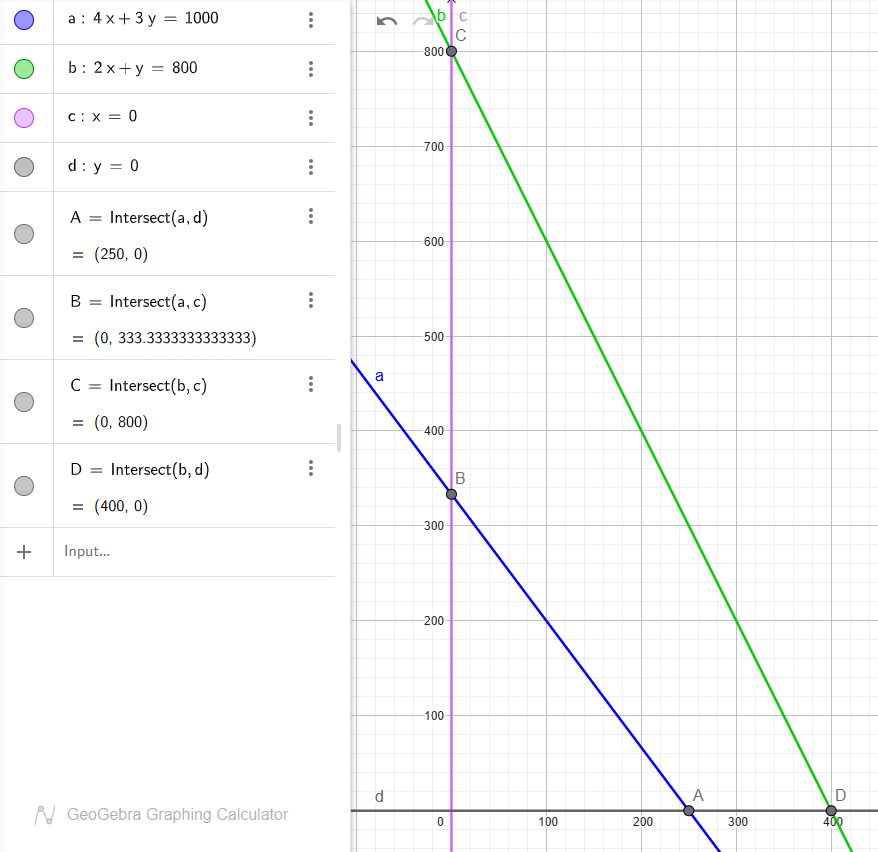
\includegraphics[width=0.6\linewidth]{assChap1-B-1.png}
        \end{center}
        จะได้ว่าบริเวณความเป็นไปได้ (feasible region) คือรูปสามเหลี่ยมที่ปิดล้อมด้วยแกน $x$, แกน $y$ และเส้นตรงสมการ $4x+3y=1000$ ซึ่งมีจุดยอด 3 จุดได้แก่ $(0,0), (0,1000/3), (250,0)$ (เนื่องจากในข้อนี้ไม่มีการตัดกันของเส้นสมการเงื่อนไขในบริเวณที่สนใจ จึงไม่มีการแก้ระบบสมการเพื่อหาจุดตัด)
    
        สุดท้ายคือแทนค่าจุดมุมลงในฟังก์ชันจุดประสงค์เพื่อหาค่าแล้วเปรียบเทียบกันว่าจุดใดให้ค่าจุดประสงค์มากที่สุด
    
        \begin{center}
            \begin{tabular}{c|c}
                $(x,y)$ & $\text{ยอดขาย} = 2000x + 1500y$ \\
                \hline
                $(0,0)$ & 0 \\
                \hline
                $(0,1000/3)\approx(0,333)$ & $499500$ \\
                \hline
                $(250,0)$ & $500000$ \\
                \hline
            \end{tabular}
        \end{center}
        ซึ่งทำให้ได้ว่าค่ายอดขายสูงสุดที่จะทำได้ภายใต้เงื่อนไขที่กำหนดมาคือ $500,000$ บาท ที่จะผลิตโต๊ะอย่างเดียว $250$ ตัว
        \begin{remark}
            {}{}
            ถ้าไม่นับเรื่องการปัดให้เป็นจำนวนเต็มนั้น จริงๆ แล้วที่จุด $(0,1000/3)$ ก็ให้ค่ายอดขายสูงสุดเป็น $500000$ บาทเช่นกัน แต่ว่าเนื่องจากเราต้องปัดให้เป็นจำนวนเต็ม และไม่สามารถปัดขึ้นได้เนื่องจากจะเกินเงื่อนไขที่กำหนดมา ทำให้เราสามารถผลิตได้ยอดขายแค่ $499500$ ที่จุดที่จะผลิตตู้อย่างเดียว\\
    
            นอกจากนั้น ทุกจุดบนเส้นสมการเงื่อนไข $4x+3y=1000$ นั้นต่างให้ค่าฟังก์ชันจุดประสงค์เป็น $500000$ เหมือนกันทุกจุด (เป็นโจทย์ทิ้งไว้ให้นักศึกษาลองคิดว่าทำไมถึงเป็นเช่นนั้น) ดังนั้น เราอาจจะเลือกตัวเลือกอื่นที่ไม่ใช่จุดมุมก็ได้ ตราบใดที่ยังเป็นจุดที่ทั้ง $x$ และ $y$ ต่างเป็นจำนวนเต็มและยังอยู่บนเงื่อนไขดังกล่าว (ตัวอย่างเช่น $x = 100, y=250$ ก็เป็นอีกจุดที่ยังสอดคล้องเงื่อนไขของโจทย์และให้ค่ายอดขายรวมเป็น $500000$ เช่นเดียวกัน)\\
    
            \textbf{โจทย์ Challenge}
            \begin{align*}
                \max \quad & 2000x + 1500y \\
                \texttt{subject to} \quad
                & 4x + 3y \leq 1000 \\
                & 2x + y \leq 800 \\
                & x \geq 0, \quad y \geq 0 
            \end{align*}
            \begin{enumerate}
                \item ทำไมทุกจุดบนเส้นเงื่อนไข $4x + 3y = 1000$ ถึงทำให้ค่ายอดขายรวมได้ราคา $500,000$ บาทเหมือนกันทั้งหมด
                \item ถ้าเกิดทางบริษัท ABC Furniture ไม่ต้องการตัวเลือกที่ผลิตแค่อย่างใดอย่างหนึ่งเท่านั้น แต่ให้ช่วยลิสต์รายการทั้งหมดที่เป็นไปได้ที่ทำให้ยอดขายรวมได้ $500,000$ บาทเหมือนกัน เราจะมีวิธีการหาตัวเลือกทั้งหมดนั้นอย่างไร\\
                (คำใบ้ $x = 250 - \frac{3}{4}y$)
            \end{enumerate}
        \end{remark}
    \end{solution}
    
    

    \item หาผลเฉลยด้วยวิธี Simplex method
    \item จงอธิบายความหมายทางเรขาคณิตของแต่ละ simplex tableau ที่ได้ในข้อที่ผ่านมา
    \item หาผลเฉลยด้วย Excel Solver
    \item ถ้าบริษัทเพิ่มแรงงานได้เป็น 1,200 ชั่วโมงต่อสัปดาห์ ข้อจำกัดเปลี่ยนแปลงอย่างไร และคำตอบใหม่คืออะไร?
    \item ถ้าราคาขายตู้เก็บเอกสารเพิ่มเป็น 1,800 บาท จะมีผลต่อคำตอบอย่างไร? ควรผลิตเปลี่ยนไปหรือไม่?
\end{enumerate}

\subsection*{Part C: Sensitivity Analysis}
เราสามารถลด (หรือเพิ่ม) ทรัพยากรได้แค่ไหน โดยที่คำตอบที่ดีที่สุด (optimal solution) ยังไม่เปลี่ยน?
\begin{enumerate}
    \item อธิบายเงื่อนไขเชิงเรขาคณิตที่ทำให้คำตอบที่เหมาะสมที่สุดยังคงอยู่ที่เดิม เมื่อเปลี่ยนค่าด้านขวาของข้อจำกัด (RHS)
    \item พิจารณาว่าเราสามารถลดค่าของ RHS ของข้อจำกัดแรงงาน (1000) และวัตถุดิบ (800) ลงอย่างละเท่าไร โดยที่จุดคำตอบเดิมยัง feasible และยังเป็นคำตอบที่ให้ค่า Z มากที่สุด
\end{enumerate}

